\documentclass[10pt, a4paper]{report}
\usepackage[utf8]{inputenc}
\usepackage{eso-pic} % \AddToShipoutPicture
\usepackage{graphicx} % \includegraphics
\usepackage{listings} % \includegraphics
\usepackage{pgfplots}
\usepackage{hyperref}
\usepackage[utf8]{inputenc}
\usepackage{mdframed}
\usepackage{float}
\usepackage{amsmath}
\usepackage{flafter}
\usepackage{graphicx}
\usepackage{tikz}
\usepackage{blindtext}
\usepackage{pgfplots}
\usepackage{seqsplit}
\usepackage[cache=false]{minted}
\usepackage{listings}
\usepackage[htt]{hyphenat}
\usepackage{amsmath,amssymb,amsbsy}
\usepackage{graphicx}
\usepackage{amsmath,amssymb,amsbsy}
\usepackage{stmaryrd}
\usepackage{semantic}
\usepackage{url}
\usepackage{color}
\usepackage{flushend}
\usepackage{subcaption}
\usepackage{tikz}
\usepackage{svg}
\usepackage{pdfpages}
\usepackage{titling}
\usepackage[parfill]{parskip}

\newcommand{\fshark}{{\texttt{FShark}}}
\newcommand{\fsharp}{{\texttt{F\#}}}
\newcommand{\csharp}{{\texttt{C\#}}}
\newcommand{\fsharpexpr}{\texttt{FSharpExpr}}

\setminted{fontsize=\small,baselinestretch=1,frame=lines,framerule=0.3pt}
\lstset{basicstyle=\small,frame=lines}
\usepackage[english, science, titlepage]{ku-frontpage}

\title{FShark}
\assignment{Master's thesis}
\author{Mikkel Storgaard Knudsen}

\subtitle{Futhark programming in FSharp}
\date{Handed in: \today{}}
\advisor{Advisor: Cosmin eller Troels}
\frontpageimage{hedgehogshark_cropped.jpg}

\author{Mikkel Storgaard Knudsen}

\usepackage{tcolorbox}
\usepackage{etoolbox}
%\BeforeBeginEnvironment{minted}{\begin{tcolorbox}}%
%\AfterEndEnvironment{minted}{\end{tcolorbox}}%

% Futhark syntax highlighting setup
\usepackage{listings}
\renewcommand{\ttdefault}{pcr} % Courier instead of Computer Modern
% Fix dashes in listings (from
% https://tex.stackexchange.com/questions/33185/listings-package-changes-hyphens-to-minus-signs
% )
\makeatletter
\lst@CCPutMacro\lst@ProcessOther {"2D}{\lst@ttfamily{-{}}{-{}}}
\@empty\z@\@empty
\makeatother
\lstdefinelanguage{Futhark}
{keywords={fun,if,then,else,loop,do,map,reduce,reduceComm,filter,scan,redomap,redomapComm,transpose,reshape,iota,replicate,let,in,for,while,with,f32,int,zip,streamSeq,zipWith,unsafe,streamRed,streamMap,mapPerThread,fn,reduceKernel,concat,split,size},%
  sensitive=true,
  comment=[l]{--},
  moredelim=**[is][\color{blue}]{$}{$}
}
\lstdefinelanguage{tail}
{keywords={let,in},%
  sensitive=true,
  comment=[l]{--},
  moredelim=**[is][\color{blue}]{$}{$}
}
\lstset{
  language=Futhark,
  basicstyle=\ttfamily,
  keywordstyle=\bfseries,
  showlines=true,
  columns=fullflexible,
  keepspaces=true,
}
% for adjustwidth environment
\usepackage[strict]{changepage}

% for formal definitions
\usepackage{framed}

% environment derived from framed.sty: see leftbar environment definition
\definecolor{formalshade}{rgb}{0.95,0.95,1}

\newenvironment{formal}{%
  \def\FrameCommand{%
    \hspace{1pt}%
    {\color{formalshade}\vrule width 4pt}%
    \colorbox{formalshade}%
  }%
  \MakeFramed{\advance\hsize-\width\FrameRestore}%
  \noindent\hspace{-4.55pt}% disable indenting first paragraph
  \begin{adjustwidth}{}{7pt}%
  \vspace{2pt}\vspace{2pt}%
}
{%
  \vspace{2pt}\end{adjustwidth}\endMakeFramed%
}

\newcommand{\evals}[1]{\llbracket #1 \rrbracket}
\newcommand{\evalfn}[1]{\evals{#1}_{\textrm{fn}}}
\newcommand{\evalbinop}[1]{\evals{#1}_{\textrm{binop}}}
\newcommand{\evalunop}[1]{\evals{#1}_{\textrm{unop}}}
\newcommand{\id}[1]{\emph{#1}}
\newcommand{\lit}[1]{\text{\ttfamily #1}} % literal

\definecolor{rosso}{RGB}{220,57,18}
\definecolor{giallo}{RGB}{255,153,0}
\definecolor{blu}{RGB}{102,140,217}
\definecolor{verde}{RGB}{16,150,24}
\definecolor{viola}{RGB}{153,0,153}

\makeatletter

\tikzstyle{chart}=[
    legend label/.style={font={\scriptsize},anchor=west,align=left},
    legend box/.style={rectangle, draw, minimum size=5pt},
    axis/.style={black,semithick,->},
    axis label/.style={anchor=east,font={\tiny}},
]

\tikzstyle{bar chart}=[
    chart,
    bar width/.code={
        \pgfmathparse{##1/2}
        \global\let\bar@w\pgfmathresult
    },
    bar/.style={very thick, draw=white},
    bar label/.style={font={\bf\small},anchor=north},
    bar value/.style={font={\footnotesize}},
    bar width=.75,
]

\tikzstyle{pie chart}=[
    chart,
    slice/.style={line cap=round, line join=round, very thick,draw=white},
    pie title/.style={font={\bf}},
    slice type/.style 2 args={
        ##1/.style={fill=##2},
        values of ##1/.style={}
    }
]

\pgfdeclarelayer{background}
\pgfdeclarelayer{foreground}
\pgfsetlayers{background,main,foreground}


\newcommand{\pie}[3][]{
    \begin{scope}[#1]
    \pgfmathsetmacro{\curA}{90}
    \pgfmathsetmacro{\r}{1}
    \def\c{(0,0)}
    \node[pie title] at (90:1.3) {#2};
    \foreach \v/\s in{#3}{
        \pgfmathsetmacro{\deltaA}{\v/100*360}
        \pgfmathsetmacro{\nextA}{\curA + \deltaA}
        \pgfmathsetmacro{\midA}{(\curA+\nextA)/2}

        \path[slice,\s] \c
            -- +(\curA:\r)
            arc (\curA:\nextA:\r)
            -- cycle;
        \pgfmathsetmacro{\d}{max((\deltaA * -(.5/50) + 1) , .5)}

        \begin{pgfonlayer}{foreground}
        \path \c -- node[pos=\d,pie values,values of \s]{$\v\%$} +(\midA:\r);
        \end{pgfonlayer}

        \global\let\curA\nextA
    }
    \end{scope}
}

\newcommand{\legend}[2][]{
    \begin{scope}[#1]
    \path
        \foreach \n/\s in {#2}
            {
                  ++(0,-10pt) node[\s,legend box] {} +(5pt,0) node[legend label] {\n}
            }
    ;
    \end{scope}
}

\begin{document}

%%%% CHAPTERS
\chapter{Prelude}

%%% Local Variables:
%%% mode: latex
%%% TeX-master: "../thesis"
%%% End:
\chapter{Introduction}
Developers worldwide are, and have always been, on the lookout for increased
computing performance.
Until recently, the increased performance could easily be
achieved through advances within raw computing power, as CPU's had steadily been
doubling their number of on-chip transistors, in rough accordance to Moore's Law (citér
her).

As performance increases in single-CPU design has stalled due to the power
wall\cite{powerwall} (among other things), developers are turning to multi-core
processors instead. As the number of cores increases, so does the number of
active threads available for parallel data processing.

Modern mainstream GPUs can run tens of thousands of threads in
parallel. Modern mainstream CPUs, like the current Ryzen series by AMD, usually
support between 10 and 20 simultaneous threads.
This makes GPUs the optimal target for data-parallel programming.

GPU programming is complicated: GPU-targeting developers must not only
write the computational kernels for the GPUs, but also often manually handle the
memory allocations and -transfers between the main program and the GPU device.
Such difficulties in GPU development, compared to normal (sequential) CPU
development, severely hinders the adaption of GPU programming in general.

Even though most programming languages support GPU programming through various
libraries, there are very solutions that offers GPU programming through high
level programming \-- the users still have to write their own kernels in some
form, and likewise declare their own buffers.

Two mainstream languages which lack high level GPU programming solutions are
\csharp{} and \fsharp{}. 

It is safe to say that there exists plenty of \csharp{} and \fsharp{} projects
in the real world, which could greatly benefit from parallelizing parts of their
algorithms, but current solutions would then demand that those parts in
particular
should be rewritten at least partly as GPU code, depending on the libraries
used. Depending on someone to have non-mainstream GPU coding skills on a
conventional developer team is not feasible, so the benefits from parallelizing
are often left alone in favor of maintaining a more accessible code base.
\clearpage

Currently, there does exist plenty of high level solutions to this problem.
In particular, numerous domain specific languages exists that allows programmers
to solve their domain specific problems in a high level language, and compile it
to standalone GPU accelerated libraries or programs.

Of such DSLs we have for instance:
\begin{itemize}
\item Forma
\item Ebb
\item one more
\end{itemize}

However, DSLs such as these are always either embedded in some host language
(such as Accelerate), or compiled to standalone executable programs. Their
compilers are designed to optimize performance, but rarely to support
interoperability to any significant degree.

Projects like APLtail\cite{apltail} have shown new ways to obtain GPU-accelerated
executables and libraries from source code written in  high level language. APLtail parses
and compiles APL\footnote{more accurately a subset of the APL language} code into redistributable C or Python libraries.

In summary, the hardware for massively parallel programming is widely available.
Furthermore, solutions exists for writing efficient GPU programs in high level
languages, but these have weak interoperability support with mainstream
languages.

\section{What \fshark{} sets out to do}
This thesis takes inspiration from APLtail\cite{apltail}, and creates a solution
that lets users compile efficient GPU programs from a high level programming
language, whilst at the same time supporting a high level of interoperability
with a mainstream language.
Whereas APLtail allows integration of GPU Futhark-written computation kernels in
C- and Python programs (by means of code generation), we would like to use code generation to make Futhark-written kernels available for use in \csharp{} and \fsharp{} programs.

To show that this is feasible, we first design a \csharp{} code generator for the
Futhark compiler. This code generator must be able to generate \csharp{} source
files, that can be compiled and used either as standalone executables, or as
importable libraries in any other \csharp{} or \fsharp{} program.
There were several notable challenges in this process, namely 1) designing
\csharp{} programs that could encapsulate entire Futhark programs in a single
class, and 2) designing helper libraries to include in the generated code, and
3) designing a way to write sequential (non-GPU) Futhark code as pure \csharp{},
in cases where GPU devices are unavailable.

The code generator alone should not convince anyone that we are creating GPU
kernels from a high level language, which is why we also design and implement a
compiler which takes source code written in a mainstream language, compiles it
as efficient GPU kernels, and (together with the code generator) makes the
resulting GPU program immediately operable from the mainstream language itself.  
The main challenges for this was 1) identifying which parts of the \fsharp{}
language that were suitable for Futhark translation, 2) implementing a standard
library for Futhark targeted \fsharp{} programs, and 3) designing and implementing a compiler
pipeline that would let users program and use GPU kernels in \fsharp{}, without
manually using Futhark compilers or importing external libraries.

Empirical evaluation demonstrates that this approach is feasible.
We both show that that unit tests written in a high level language can be compiled and executed
correctly as computational kernels on the GPU, just as we also take complex
benchmark programs written in a mainstream language, compile them into
computational kernels for the GPU, and use them directly in the mainstream
language afterwards.







\section*{Motivation}
\fshark{} is intended to be a way of writing and utilizing Futhark, without
actually having to write or interact with the Futhark language and compiler
itself. Besides some tooling and an \fsharp{} SOAC library, it primarily consists of the \fshark{} compiler that compiles from
\fsharp{} source code to Futhark source code, and the Futhark \csharp{}
generator, which compiles Futhark programs as either standalone \csharp{}
programs or -libraries.

As much as most developers are happy to increase performance on big
computations, it is not always an option to incorporate an extra langauge into
an already existing programming language. At this moment, using Futhark in
either a \csharp{}- or \fsharp{} project is a contrived process that usually
requires spawning a subprocess with a \texttt{futhark-opencl} C program from inside one of the .NET
projects.

In order to use Futhark natively in .NET languages, it is therefore
necessary to write a backend for Futhark in a .NET language.
For \fshark{}, I have chosen to implement this backend in \csharp{}, as the Futhark intermediate
code \texttt{ImpCode}\footnote{which stands for Imperative Code} is trivial to
translate into imperative \csharp{} statements and expressions.
Also, there are \csharp{} libraries available which supply OpenCL bindings, which are
needed to implement the necessary OpenCL constructs from \texttt{ImpCode}.

It is my belief that exporting Futhark programs as .NET executables and
-libraries will lower the barrier to Futhark usage in .NET projects
significantly, hopefully increasing the all-round number of Futhark users, and
in the long term, increasing utilization of GPU programming and making it more
widely available.

However, one could do even more than just exporting Futhark to .NET, to increase
accessibility:

As tens of thousands of programmers worldwide (CHECK NUMBER JEEEEZ) are already
writing \fsharp{} programs, and that most of \fsharp{}s functional language features can be
directly translated into equivalent Futhark features, it became worthwhile to
investigate whether it was possible to design a way for users to both write and
utilize Futhark in \fsharp{} projects, without ever actually touching the
Futhark language or compiler themselves.
Instead, users can write their data parallel \fsharp{} modules in \fshark{}, and compile these
modules into Futhark libraries automatically.

In this case, it would be possible to get Futhark speeds in \fsharp{} programs,
without doing much more than installing the Futhark compiler locally, and adding
the required \fshark{} libraries to the \fsharp{} project.

It is my belief that being able to achieve Futhark performance in regular \fsharp{}
programs almost automatically, will make it significantly easier for people to
adapt to Futhark programming.

(SOME MORE MORE SOME MORE)

\clearpage

\section*{The contributions of this thesis}
The contributions of this thesis are as follows:
\begin{enumerate}
\item A \csharp{} code generator for the Futhark language compiler, which
  generates GPU accelerated libraries that can integrate seamlessly in 
  \csharp{} and \fsharp{} code bases.

\item A select subset of the \fsharp{} langauge which can be translated directly to
  Futhark source code of equivalent functionality. This includes a
  library which implements Futhark SOACs\cite{soacs} in \fsharp{}, allowing
  people to write \fsharp{} code which can be ported automatically to Futhark.

\item A compiler and wrapper pipeline which allows users to compile individual
  \fsharp{} modules in their projects to GPU accelerated libraries, and load and
  execute code from these modules in the rest of the \fsharp{} project.

\item A set of benchmarks and unit tests that shows that this approach is indeed feasible.
\end{enumerate}

\clearpage
\section*{Vocabulary}
Unless otherwise specified, these are the terms used in the thesis:
\begin{description}
\item[For \fshark{}]\hfill
  \begin{itemize}
  \item The \fshark{} \textit{subset} is the subset of the \fsharp{} language
    that is supported by the \fshark{} compiler.

  \item The FShark Prelude is the library of \fsharp{}-ported Futhark array
    functions and SOACs, and is included with \fshark{}.

  \item \fshark{} code is \fsharp{} code which exclusively uses the \fshark{}
    subset and FSharkPrelude.

  \item \fshark{} modules are \fsharp{} modules written entirely in \fshark{}
    code.
    
  \item \fshark{} projects are \fsharp{} projects which uses \fshark{} and
    \fshark{} modules.
    \\
  \end{itemize}

\item[For Futhark]\hfill
  \begin{itemize}

  \item Futhark code is code written in Futhark.

  \item Futhark C-, Python- or \csharp{} code refers to Futhark code that has been compiled
    into C-, Python or \csharp{} source code.

  \end{itemize}
\end{description}



\section*{Roadmap}
The main part of this thesis is split in four parts.
blaaaah


%%% Local Variables:
%%% mode: latex
%%% TeX-master: "../thesis"
%%% End:
\chapter{Background}
\fshark{} is built on the interaction between Futhark, \fsharp{} and \csharp{},
wherefore WE SHOULD HAVE A BETTER INTRODUCTION FOR THIS CHAPTER.

\section{\fsharp{}}
\fsharp{} is a relatively young .NET-based language, first released in 2003.
It is a strongly-typed multiple-paradigm language, with a syntax that is
primarily functional, resembling OCaml.
Although \fsharp{} is not as widely used as \csharp{}, \texttt{Java} and the
like, it is currently experiencing increasing adaptation among
developers\cite{citeme}.
Besides supporting multiple paradigms and a reasonable subset of functional
langauge features (such as pattern matching), \fsharp{}s primary strength is
it's interoperability with the rest of the .NET ecosystem. Like \csharp{},
\fsharp{} programs are compiled into Microsoft's \texttt{Common Intermediate
  Langauge}, and executed using Microsoft's \texttt{Common Language Runtime}.

Therefore, \fsharp{} programs have full access to the standard .NET library,
just as it can also readily import and use classes and methods from arbitrary
\csharp{} libraries.

For \fshark{}, \fsharp{} has been selected as a source language for several
reasons.
First, most of \fsharp{}s syntax is readily translatable into Futhark syntax, as
long as the programmer stays away from using any of \fsharp{}s non-functional
constructs, like \texttt{async} or it's object oriented features.
Second, as \fsharp{} effortlessly interoperates with \csharp{} programs, and
\csharp{} has plenty of OpenCL libraries available, we can write imperative
OpenCL-powered programs in \csharp{}, for use in \fsharp{} projects.
%% written example


\section{Futhark}
Quoting from Futhark's own homepage,
\begin{formal}
  Futhark is a small programming language designed to be compiled to efficient parallel code. It is a statically typed, data-parallel, and purely functional array language in the ML family, and comes with a heavily optimising ahead-of-time compiler that presently generates GPU code via OpenCL, although the language itself is hardware-agnostic.
\end{formal}
So far, plenty of handwritten GPU benchmark programs implemented in CUDA et al,
has been ported to Futhark, with significant performance gains as a result.
\cite{citesomething}. With these results in mind, it makes sense to start
implementing other parallelizable algorithms and programs in Futhark. However,
in the grand scheme of things, Futhark is still a relatively obscure programming
language, and is almost solely used in academic settings.

With Futhark being a purely functional programming language, it has very few
imperative language constructs available, and the few that it has, like
in-place updates, are merely syntactic sugar for other existing library function calls.

As Futhark's main functionality is generating OpenCL kernels, it is in principle
possible to compile Futhark programs for any language that are able to interface
with the OpenCL API.

%err, måske flytte eller skrive om
As a target language for \fsharp{} translations,
Futhark is ideal as we can identify and relatively easily translate a subset
of the \fsharp{} language to equivalent Futhark code, as the syntax itself is
very similar. Even though \fsharp{} also allows plenty of imperative and object
oriented programming,
\fshark{} blocks the user from using these constructs, by failing at \fshark{}
compile time.

% måske tilføje noget om unsafe

\section{\csharp{}}
\csharp{} 
\csharp{} 
\csharp{} 
\csharp{} 




%%% Local Variables:
%%% mode: latex
%%% TeX-master: "../thesis"
%%% End:

\chapter{The \fshark{} language}
In this chapter we present the \fshark{} language and it's standard library.
We start out by presenting \fshark{}'s syntax and discussing the syntax's
limitations.
Afterwards we present first the built-in \fsharp{} operators and \fsharp{}
standard library functions available in \fshark{}.
We then present our own standard library written specifically for \fshark{}, and
discuss why we implemented our own standard library instead of using the
standard library already available in \fsharp{}.

Then, we discuss how array types are implemented in \fshark{}, and how
\fsharp{} arrays differ from Futhark arrays.
Finally, we describe and solve the implementation challenges caused by our
design choices, and discuss alternative solutions to the one that was chosen.

\section{What the \fshark{} language is}
\label{chap:fsharklanguage}
The second contribution of this thesis is a high level programming language,
which can be compiled automatically to GPU kernels that are readily usable in
a mainstream programming language.

The \fshark{} language is the sum of two parts: \\
1) The \fshark{} subset, which is a defined subset of the \fsharp{} language and
the \fsharp{} standard library.\\
2) An accompanying standard library, which adds SOACs and array functions that
can be used in programs written in the \fshark{} subset.

The \fshark{} language can be compiled into standalone GPU kernels using the
\fshark{} compiler \ref{chap:fsharkcompiler}. These kernels can then be integrated directly in
\fsharp{} programs.

The program in figure \ref{fig:shortfsharkprogram0'} is written in \fshark{},
and can be used as any other \fsharp{} code in an \fsharp{} project.
However, as it is written in \fshark{}, we can pass it through the \fshark{}
compiler and end up with the result Futhark code shown in figure \ref{fig:shortfsharkprogram1'}
At this moment we we will skip explaining the meaning of the code, and simply
point out that the \fshark{} source code and the resulting source code have a
strong resemblance.
\begin{figure}[H]
  \centering
\begin{minted}{fsharp}
let saxpy (a : int) (x : int) (y : int) : int =
  a*x+y

let getArrayPair (a : int) : (int array * int array) =
  let xs = Iota a
  let n = Length xs
  let ys = Rotate (a / n) xs
  in (xs, ys)

[<FSharkEntry>]
let entry (a : int) : int array =
  let (xs, ys) = getArrayPair a
  let res = Map2 (saxpy a) xs ys
  in res
\end{minted}
  \caption{A short \fshark{} program}
  \label{fig:shortfsharkprogram0'}
\end{figure}

\begin{figure}[H]
  \centering
  \begin{lstlisting}[language=Futhark, breaklines]
let saxpy (a : i32) (x : i32) (y : i32) : i32 =
  ((((a * x)) + y))
let getArrayPair (a : i32) : ([]i32, []i32) =
  let xs = iota (a)  in
  let n = length (xs)  in
  let ys = rotate (((a / n))) (xs) in
  (xs, ys)
entry entry (a : i32) : []i32 =
  unsafe let patternInput = getArrayPair(a) in
         let ys = patternInput.2 in
         let xs = patternInput.1 in
         let res = map2 ((\(x : i32) -> (\(y : i32) -> saxpy(a) (x) (y)))) (xs) (ys) in
         res
\end{lstlisting}
  \caption{The source code in figure \ref{fig:shortfsharkprogram0'} compiled to
    Futhark source code by the \fshark{} compiler.}
  \label{fig:shortfsharkprogram1'}
\end{figure}

In the following section, we will describe the entire \fshark{} language. Although the
subset is just a part of \fsharp{}, we will describe it as if it was a new language.

\clearpage
\section{\fshark{} syntax}
\Cref{fig:fsharkstatements,fig:fsharkexpressions,fig:fsharkpatterns,fig:fsharktypes,fig:fsharkliterals}
shows the complete \fshark{} syntax.

\begin{figure}[h]
  \centering
  \begin{tabular}{lclr}
    $prog$ & $::=$ & $module\ prog$ & \\
           & $|$   & $prog'\ prog$  & \\
           & $|$   & $\epsilon$     & \\

    $prog'$ & $::=$ & $typealias$   & \\
            & $|$   & $fun$ & \\

    $progs'$ & $::=$ & $prog'\ progs'$   & \\
             & $|$   & $\epsilon$ & \\
    \\
    $typealias$ & $::=$ & $\texttt{type}\ v\ = t $& \\
    $module$ & $::=$ & $\texttt{module}\ v = prog'\ progs'$ & \textit{(See subsec \ref{noteonfsharkmodules} on \fshark{} modules)} \\
    \\
  \end{tabular}
  \begin{tabular}{lclr}
    $fun$ & $::=$ & \texttt{[<FSharkEntry>]} $\texttt{let}\ id\ (v_1 : t_1)\ \ldots\ (v_n : t_n) : t = e$ & \\
        & $|$   & $\texttt{let}\ v\ (v_1 : t_1)\ \ldots\ (v_n : t_n) : t' = e,$ & \textit{{See subsec \ref{noteonfsharktypes}}}  \\
    \\

  \end{tabular}
  \caption{\fshark{} statements}
  \label{fig:fsharkstatements}
\end{figure}



\begin{figure}[h]
  \centering
  \begin{tabular}{lclr}
    $e$ & $::=$ & $(e)$ & (Expression in parenthesis) \\
        & $|$   & $k$ & (Constant) \\
        & $|$   & $v$ & (Variable) \\
        & $|$   & $(e_0,~\ldots,~e_n)$ & (Tuple expression) \\
        & $|$   & $\{\texttt{id}_0=e_0 ; \ldots ; \texttt{id}_n=e_n\}$ & (Record expression) \\
        & $|$   & $[\vert e_0 ; \ldots ; e_n\vert]$ & (Array expression) \\
        & $|$   & $v.[e_0] \ldots .[e_n]$ & (Array indexing) \\
        & $|$   & $v.id$ & (Record indexing) \\
        & $|$   & $v.id$ & (Module indexing (\textit{See subsec \ref{noteonfsharkmodules}})) \\
        & $|$   & $e_1 \odot e_2$ & (Binary operator) \\
        & $|$   & $-e$ & (Prefix minus) \\
        & $|$   & \texttt{not} $e$ & (Logical negation) \\
        & $|$   & \texttt{if} $e_1$ \texttt{then} $e_2$ \texttt{else} $e_3$ & (Branching) \\
        & $|$   & \texttt{let} $p = e_1$ \texttt{in} $e_2$ & (Pattern binding) \\
        & $|$   & $\mathtt{fun}~p_0~\ldots~p_n~\mathtt{->}~e$ & (Anonymous function) \\
        & $|$   & $e_0~e_1$ & (Application) \\

    \\
  \end{tabular}
  \caption{\fshark{} expressions}
\label{fig:fsharkexpressions}
\end{figure}

\begin{figure}[h]
  \centering
  \begin{tabular}{@{}lclr}
    $p$ & $::=$ & $id$ & (Name pattern) \\
        & $|$   & $(p_0, \ldots, p_n)$ & (Tuple pattern) \\
  \end{tabular}
  \caption{\fshark{} patterns}
\label{fig:fsharkpatterns}
\end{figure}



\begin{figure}[h]
  \centering
  \begin{tabular}{@{}lclr}
    $t$ & $::=$ & $\texttt{int8}~|~\texttt{int16} ~|~ \texttt{int} ~ |~\texttt{int64} $ & (Integers) \\
        & $|$   & $\texttt{uint8} ~ | ~\texttt{uint16} ~|~\texttt{uint} ~|~\texttt{uint64} $ & (Unsigned integers) \\
        & $|$   & $\texttt{single} ~| ~\texttt{double}$ & (Floats) \\
        & $|$   & $\texttt{bool}$ & (Booleans) \\
        & $|$   & $(t_0 * \ldots * t_n)$ & (Tuples) \\
        & $|$   & $\{id_0:t_0;~\ldots;~id_n:t_n\}$ & (Records) \\
        & $|$   & $t~\mathtt{array}$& (Arrays) \\
    \\
  \end{tabular}
  \caption{\fshark{} types}
\label{fig:fsharktypes}
\end{figure}

\begin{figure}[h]
  \centering
  \begin{tabular}{@{}lclr}
    $k$ & $::=$ & $n\lit{y}~|~n\lit{s}~|~n~|~n\lit{L}$ & (8-, 16-, 32- and 64 bit signed integers) \\
        & $|$   & $n\lit{uy}~|~n\lit{us}~|~n~|~n\lit{UL}$ & (8-, 16-, 32- and 64 bit unsigned integers) \\
        & $|$   & $d\lit{f}~|~d $ & (Single and double precision floats) \\
        & $|$   & $true~|~false$ & (Boolean) \\
        & $|$   & $(k_0 ,~\ldots ,~k_n)$ & (Tuple) \\
        & $|$   & $\{id_0=k_0;~\ldots;~id_n=k_n\}$ & (Record) \\
        & $|$   & $[\vert k_0 ; \ldots ; k_n\vert]$ & (Array literals) \\
    \\
  \end{tabular}
  \caption{\fshark{} literals}
\label{fig:fsharkliterals}
\end{figure}
\clearpage
\section{Notes to the \fshark{} grammar}
\subsection{Limits to function argument types}
\label{noteonfsharktypes}
There are several limits to the \fsharp{} compiler, which limits the types
available in function definitions.\\
\begin{enumerate}
\item Tuples in entry functions, whether they are used in the arguments or in the
return types, are allowed to contain a maximum of seven elements. This is
because the CLR runtime uses the type \texttt{System.Tuple} for these tuples.
Incidentally, \texttt{System.Tuple} is only defined for tuples up to seven
elements.

This limitation can be circumvented by using more tuples. For example, rewriting
a function so it returns \\
\texttt{((int * int * int * int) * (int * int * int * int))}\\
instead of\\
\texttt{(int * int * int * int * int * int * int * int)}.

\item Non-entry functions cannot have tuple type arguments.
  For functions that take tuple arguments, the \fsharp{} compiler parses these
  tuple type arguments correctly.
  However, the \fsharp{} compiler rewrites calls to these functions in a curried
  way. Figure~\Cref{fig:astcurried} shows two two \fsharp{} functions, {\tt foo}
    and {\tt bar}, and figure~\Cref{fig:astcurried'} shows a simplified 
    representation of how these functions are represented in the
    \fsharp{}-compiler intermediate representation.

  When translating from \fshark{} to Futhark, the Foo function is correctly
  written in Futhark as a function with a tuple argument, but since the call
  expression {\tt Call foo 4 5} now treats \texttt{foo} as having a different 
  type than first defined, the corresponding Futhark translation will trigger 
  a type error at compile time.

\begin{figure}[H]
\centering
\begin{minted}{fsharp}
let foo ((x , y) : (int * int)) : int = x + y

let bar = foo (4,5)
\end{minted}
\caption{A function calling another function in \fsharp{}}
    \label{fig:astcurried}
    \end{figure}
\begin{figure}[H]
\begin{minted}{lisp}
Function foo ((x , y) : (int * int)) : int = x + y

Function bar () : int = Call foo 4 5
\end{minted}
    \caption{\fsharp{} compiler curries tuple arguments when calling tuple functions}
    \label{fig:astcurried'}
  \end{figure}

\item Entry functions should not use record type arguments, as these have not
  been investigated fully for \fshark{} use yet.
\end{enumerate}

\subsection{\fshark{} modules}
\label{noteonfsharkmodules}
The modules supported in \fshark{} are not higher-order modules as in
\texttt{ML}, but instead just a nested namespace in the containing module.

\section{\fsharp{} operators available in \fshark{}}
The \fsharp{} subset chosen for \fshark{} is described in \ref{fig:fsharkops}.
Note that all of these operators are overloaded and defined for all integer
and floating point types in \fsharp{}, except for modulus which in Futhark is
only defined for integers.

\begin{figure}[h]
  \centering
\begin{description}
\item[Arithmetic operators]\hfill\\
  The set of supported arithmetic operators is addition (\texttt{+}),
  binary subtraction and unary negation (\texttt{-}), multiplication
  (\texttt{*}), division (\texttt{/}) and modulus (\texttt{\%}).

\item[Boolean operators]\hfill\\
  \fshark{} currently supports logical AND (\texttt{\&\&}), logical OR
  (\texttt{$||$}), less- and greater-than (\texttt{<}, \texttt{>}), less- and
  greater-or-equal (\texttt{<=}, \texttt{>=}), equality (\texttt{=}),
  inequality (\texttt{<>}) and logical negation (\texttt{not}).

\item[Special operators]\hfill\\
  \fshark{} also supports some of \fsharp{}s syntactic sugar. These operators
  might not have direct Futhark counterparts, but their applications can be
  rewritten in Futhark for equivalent functionality.
  The supported operators are back- and forward pipes (\texttt{<|} and
  \texttt{|>}), and the range operator ($e_0$ \texttt{..} $e_1$), which
  generates the sequence of numbers in the interval $[e_0,e_1]$.

  Note that the range operator must be used inside an array (as so
  \texttt{$[\vert e_0..e_1\vert]$}), so the expression generates an array
  instead of a list.
\end{description}
  \caption{\fshark{} operators}
\label{fig:fsharkops}
\end{figure}



\section{\fsharp{} standard library functions available in \fshark{}}
\fshark{} supports a subset of the \fsharp{} standard library. These are
readily available in all \fsharp{} programs, without having to open other modules.
The standard library subset is shown in figure \ref{fig:fsharkfuns}.
\begin{figure}[h]
  \centering
\begin{description}
\item[\texttt{id}]\hfill\\
  The identity function.

\item[Common math function]\hfill\\
  The square root function (\texttt{sqrt}), the absolute value (\texttt{abs}),
  the natural exponential function (\texttt{exp}), the natural- and the decimal
  logarithm (\texttt{log} and \texttt{log10}).
  
\item[Common trigonometric functions]\hfill\\
  Sine, cosine and tangent functions (both standard and hyperbolic):
  \texttt{sin}, \texttt{cos}, \texttt{tan}), \texttt{sinh}, \texttt{cosh} and \texttt{tanh}.
  Also one- and two-argument arctangent: \texttt{atan} and \texttt{atan2}.

\item[Rounding functions]\hfill\\
  \fshark{} supports all of \fsharp{}s rounding functions:
  \texttt{floor}, \texttt{ceil}, \texttt{round} and \texttt{truncate}.
  
\item[Number convertion functions]\hfill\\
  \fshark{} supports all of \fsharp{}s number convertion functions.
  For all the following functions $t$, $t e = e', e : t_0, e' : t$, barring
  exceptions like trying to convert a too large 64-bit integer into a 32-bit
  integer.

  The convertion functions available are \texttt{int8}, \texttt{int16}, \texttt{int}, \texttt{int64}, \texttt{uint8}, \texttt{uint16},
  \texttt{uint}, \texttt{uin64}, \texttt{single}, \texttt{double}, \texttt{bool}.
  
\item[Various common number functions]\hfill\\
  \texttt{min}, \texttt{max}, \texttt{sign} and \texttt{compare}.
\end{description}
  \caption{\fshark{} operators}
  \label{fig:fsharkfuns}
\end{figure}

\subsection{On selection the \fsharp{} subset to include in \fshark{}}
For selecting the \fsharp{} subset to support in \fshark{}, I chose to look at
what functions that were included in \fsharp{}'s prelude. That is, the
functions that are available in an \fsharp{} program without having to
\texttt{open} their containing module first.
Fortunately, \fsharp{} opens several modules by default of which I only
needed to look in two different ones, to be able to support a reasonable amount
of \fsharp{} built-ins in \fshark{}.

The primary module used in my supported \fsharp{} subset is the module
\texttt{FSharp.Core.Operators}.
This module contained not only the standard arithmetic described in figure
\ref{fig:fsharkops}, but also most\footnote{except for some convertion
  functions, found in \texttt{FSharp.Core.ExtraTopLevelOperators}} of the functions shown in the figure \ref{fig:fsharkfuns}.
Except for \texttt{unit} type functions like \texttt{failwith}, \texttt{exit}
and \texttt{async}, most of the functions and operators
\texttt{FSharp.Core.Operators} have direct counterparts in Futhark's prelude,
with equivalent functionality: All except for four of operators and functions chosen for
\fshark{} are in fact implemented in Futhark's \texttt{math.fut} library.
It was therefore an obvious decision to support these functions and operators in
\fshark{}.

However, for the remaining four functions\footnote{\texttt{compare}, \texttt{cosh}, \texttt{sinh}, \texttt{tanh}} that didn't have equivalents in
Futhark's \texttt{math.fut}, their function calls are replaced with their
identities instead.
For example, the \fshark{} code shown below:
\begin{minted}{fsharp}
  exp x
\end{minted}

can be expressed in Futhark directly as shown below:
\begin{lstlisting}[language=Futhark]
  exp x
\end{lstlisting}
\\
\\
However, the hyperbolic cosine function (shown below) is available in \fsharp{}, but not in Futhark.
\begin{minted}{fsharp}
  cosh x
\end{minted}
Therefore, the compiled \fshark{} Futhark code is just the hyperbolic function
inlined.
When the \fshark{} compiler encounters the \texttt{cosh} function the \texttt{cosh} call is replaced with
  \texttt{cosh}'s definition in the \fshark{} generated Futhark code. This is
  shown below:
  
\begin{lstlisting}[language=Futhark]
  ((exp x) + (exp (-x))) / 2.0
\end{lstlisting}

These rewritings are not pretty to look at from a programmer's perspective, but
the Futhark code generated by the \fshark{} compiler is not meant to be read by humans anyhow.

\subsection{Missing arithmetic operators in \fshark{}}
Currently, bitwise operators like bitwise-AND and bitwise-OR are missing, but
they should be relatively simple to add to the \fshark{} subset, by adding them
to the set of supported operators in the \fshark{} compiler.

\section{The \fshark{} standard library}
Besides defining an \fsharp{} subset suitable for Futhark translation, it was
also imperative to create a standard library of SOACs and array functions for \fshark{},
to make it possible to write programs with parallel higher-order array
functions.
\\
We call this standard library \texttt{FSharkPrelude}.

Similarly to how the subset of math functions chosen from \fsharp{} to include in
the \fshark{} was chosen, the SOACs and array function included in the
\texttt{FSharkPrelude} has been picked directly from the Futhark libraries
\texttt{futlib/array.fut} and \texttt{futlib/soacs.fut}. The \texttt{FSharkPrelude} doesn't
discriminate between array functions and SOACs, as maintaining and importing two
different prelude files in \fshark{} was needlessly complicated.

The \texttt{FSharkPrelude} consists of functions which are directly named after
their Futhark counterparts, and have equivalent functionality.
This prelude, together with the \fshark{} subset, is what makes up the \fshark{} language.
When \fshark{} developers are writing modules in \fshark{}, they are "guaranteed"
that their \fshark{} programs has the same results whether they are executed as
native \fsharp{} code, or compiled and executed as Futhark. 
The guarantee is on the condition that we know that the
individual parts of the \fshark{} language and standard library,  are correctly
translated to Futhark counterparts.
We can check that this condition still holds by running the \fshark{} test
suite. See sec \ref{subsec:fsharkcorrectness} for an elaboration on these tests.


The \texttt{FSharkPrelude} versions of Futhark functions are defined in three
different ways.
\begin{enumerate}
  \item Functions like \texttt{map} and array functions like
    \texttt{length} have direct \fsharp{} equivalents. The
    \texttt{FSharkPrelude} versions therefore simply pass their arguments on to
    the existing functions.
    Other functions, like the \texttt{map} functions which takes multiple arrays as
    arguments, require a bit of assembly first. For those \texttt{map} functions,
    we zip the arguments before using \texttt{Array.map} as usual.
    For example, FSharkPrelude.Map is shown in below:
\begin{minted}{fsharp}
let Map (f : 'a -> 'b) (xs : 'a array) : 'b array =
  Array.map f xs
\end{minted}

  \item Some Futhark SOACs have \fsharp{} counterparts that are very close to
    their original definition.
    for example, Futhark's \texttt{reduce} takes a neutral element\footnote{For
      parallelization purposes} as one of the
    arguments in their function calls, whilst their \fsharp{} counterparts
    (\texttt{Array.reduce}) does only take an operator and an array as
    arguments.
    In such cases, the \texttt{FSharkPrelude} version changes the input slightly
    before passing it on to the existing function. See example below:

\begin{minted}{fsharp}
let Reduce (op: 'a -> 'a -> 'a) (neutral : 'a) (xs : 'a array) =
  if null xs then neutral 
  else Array.reduce op xs
\end{minted}

  \item Lastly, some functions does not have \fsharp{} counterparts at all, such
    as scatter. In these cases, we manually implement an equivalent function in
    \fsharp{}.
    Note that we are not limited to the \fshark{} subset in the
    \texttt{FSharkPrelude}, as the prelude function calls are not translated by the
    \fshark{} compiler, but detected and exchanged for
    Futhark function calls of the same name during the \fshark{} compilation.
    \texttt{FSharkPrelude.Scatter}\footnote{The SOAC Scatter actually has limitations
      regarding \fshark{} use. See section~\ref{subsec:badscatter}} is shown below:
\begin{minted}{fsharp}
let Scatter (dest : 'a array) (is : int array) (vs : 'a array) : 'a array =
  for (i,v) in Zip is vs do
    dest.[i] <- v
  dest
\end{minted}

\end{enumerate}
The complete list of available SOACs and array functions is available in
appendix \ref{appendix:soacs}.

\subsection*{Why is FSharkPrelude part of the \fshark{} language?}
Although plenty of functions in the Futhark library already has \fsharp{}
counterparts, we have chosen not to allow these \fsharp{} counterparts to be
used directly in \fshark{} programs.
Besides basic differences like different naming in \fsharp{} and Futhark for
equivalent functions\footnote{like \texttt{fold} and \texttt{foldBack} vs.
  \texttt{foldl} and \texttt{foldr}} like, there are multiple other reasons.

1) From a user experience point of view, it is awkward to maintain a whitelist
of accepted functions from certain classes.
For example, \texttt{Array.map} is exchangable with Futhark's
\texttt{map}, but there are no immediate Futhark version of \fsharp{}s
\texttt{Array.sortInPlace}. Therefore, the \fshark{} compiler would succesfully
exchange a call to \texttt{Array.map} with a call to \texttt{map}, but it would
have to halt with an error message, if the user tried to use \texttt{Array.sortInPlace}.

2) Some Array functions have subtle differences compared to their
Futhark counterparts. As shown in \texttt{FSharkPrelude.Reduce} example,
\texttt{Array.reduce} is slightly different in \fsharp{}.

We are slightly hypocritical, as we DO let users use a subset of \fsharp{}s
standard library functions. However, there is a whitelist available for this
subset in the \fshark{} language specification, and the standard library
functions are not visibly called as a method from another module.

\subsection*{How \fshark{} SOACs differ from Futhark's ditto}
On a surface level, \fshark{} and Futhark SOACs are the same. After all, they
have equivalent functionality.
However, Futhark's SOACs gets special treatment in the Futhark compiler, and are
fused together where applicable.
Take for instance the short code example in figure \ref{fig:futharkfusion}.

\begin{figure}[h]
  \centering
\begin{lstlisting}[language=Futhark]
entry main : []f32 =
  let xs = iota 100
  let ys = map (f32.i32) xs
  let zs = map (+ 4.5f32) ys
  in zs
\end{lstlisting}
  \caption{A short Futhark program consisting of just SOACs}
  \label{fig:futharkfusion}
\end{figure}

For non-OpenCL programs, Futhark's compiler fuses all three expressions into one for-loop, as described
in simplified Futhark \csharp{} code in figure \ref{fig:pseudofusion}.
Similarly, in an OpenCL program, the short code example is translated into a
single kernel, as shown in figure \ref{fig:pseudokernel}.

\begin{figure}[h]
  \centering
\begin{minted}{csharp}
float[] mem = new float[100];
for (int i = 0 ; i < 100 ;i++)
{
  float res = int_to_float(i);
  res = res + 4.5f;
  mem[i] = res;
}
\end{minted}
  \caption{Figure \ref{fig:futharkfusion} compiled as (simplified) non-OpenCL
    \csharp{} code.}
  \label{fig:pseudofusion}
\end{figure}

\begin{figure}
  \centering
\begin{minted}{cpp}
__kernel void map_kernel(__global unsigned byte *mem)
{
   int global_thread_id = get_global_id();
   bool thread_active = global_thread_id < 100;

   float res;

   if (thread_active) {
       res = int_to_float(global_thread_id);
       res = res + 4.5f;
   }
   if (thread_active) {
       *(__global float *) &mem[global_thread_id * 4] = res;
   }
};
\end{minted}
  \caption{Figure \ref{fig:futharkfusion}, but compiled as a simplified OpenCL kernel.}
  \label{fig:pseudokernel}
\end{figure}


In both of the compiled examples, we must first allocate a target array for our
result, but note that although we obtain three different arrays in the original
Futhark code, both of the compiled versions transform the \texttt{iota}
expression into a for-loop instead, and inserts the operators from the two
subsequent \texttt{map}s into the loop.

This is a concrete implementation Futhark fusion rules as defined in \cite{pldi17}; which states
that $(map~f) \circ (map~g) \equiv map (f \circ g)$

However, executing \fshark{} code as native \fsharp{} code will execute the
expressions as written, which means that we are allocating and writing to an
array three times, once for each line in the program.

\subsubsection*{Futhark and nested maps}
Futhark's compiler also specializes in parallelizing nested SOAC
calls\cite{pldi17}, which for example transforms nested \texttt{map} expressions into one
single \texttt{map} expression. For Futhark programs like the one in figure
\ref{fig:fsharpnested}, the resulting OpenCL program contains a single map
kernel with $i * j$ active threads.

\begin{figure}[h]
  \centering
\begin{minted}{fsharp}
let xss = map (\row ->
              map (fun col ->
                row * col
              ) <| iota j
          ) <| iota i
\end{minted}
  \caption{A nested \fshark{} program}
  \label{fig:fsharpnested}
\end{figure}

The \fsharp{} compiler doesn't make any such transformations for \fshark{} programs.

\section{Arrays in \fsharp{} versus in Futhark}

As Futhark is an array language, designing the array handling for \fshark{} was
an important part of the design process.
Whereas multidimensional array types in Futhark are written as, for example,
\texttt{[][]i32} for a two dimensional integer array, their actual representation 
in the compiled code is a flat array of bytes, and an array of integers denoting 
the lengths of the dimensions.
Accessing the array at runtime can be done in $O(1)$, whether it's
either at some constant or a variable index (for example \texttt{let second\_x = xs[2]} or \texttt{let n = xs[i,j]}).
The indexes are resolved during the Futhark compilation, either as scalars, or
as a variable calculated from other variables.

Functional languages like Haskell mainly works with lists. Although \fsharp{} is
a multi-paradigm language and not exclusively functional, we primarily work with
lists when writing functional code in \fsharp{}.

In \fsharp{}, lists are implemented as singly linked lists. Nodes in the
list are dynamically allocated on the heap, and lookups take $O(n)$ time, where
$n$ is the length of the list.
We cannot make multidimensional lists, but we can make lists of lists: If we
were to emulate a two dimensional list of integers in \fsharp{}, we could use
the type \texttt{int list list}. At runtime, the type would then be realized as
a singly linked list of references to singly linked list of integers.
For an \texttt{int list list} of $n \times m$ integers, we therefore have
lookups in $O(n+m)$ time.

\fsharp{} does also have arrays. The \texttt{System.Array} class itself is reference
type.\\
If we initialize an integer array in \fsharp{} like in figure
\ref{fig:initarray0}, the result is that the variable \texttt{arr} is a reference to where it's corresponding
array is located in memory. 

As the integers contained in the array are value
types, the layout of the array referenced by \texttt{arr} is some initial array
metadata, and then the ten integers stored in sequence.
\begin{figure}[H]
  \centering
\begin{minted}{fsharp}
// Array.create : int -> 'a -> 'a array
let arr = Array.create 10 0
// arr = [|0; 0; 0; 0; 0; 0; 0; 0; 0; 0;|]
\end{minted}
  \caption{Initializing an array in \fsharp{}}
  \label{fig:initarray0}
\end{figure}
We can access the array elements on $O(1)$ time, as indexing into the array is
just done by accessing the array reference plus an index offset.
If we want to emulate multidimensional arrays with these elements, we can create
arrays of arrays (in .NET terms, these are called ``jagged arrays'').
In figure \ref{fig:jaggedarrayfsharp} we initialize a jagged array of integers.
To see how the jagged array is stored in memory, see figure \ref{fig:jaggedarraydrawing}.

\begin{figure}
  \centering
  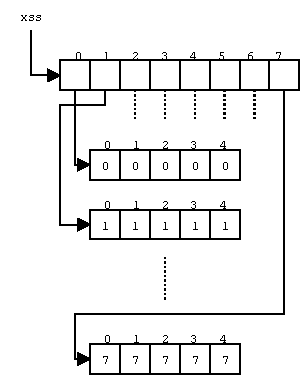
\includegraphics[scale=2]{chapters/figs/jaggedarrays.pdf}
  \caption{The memory representation of an 8 by 5 jagged array in \csharp{}.}
  \label{fig:jaggedarraydrawing}
\end{figure}


\texttt{xss} is an array of arrays, so \texttt{xss} is a reference to an array
in memory, which itself contains references to other arrays.
To retrieve the variable \texttt{some\_two}, we first follow the reference to
the array \texttt{xss} in memory. There we get the second element, which is a
reference to another array in memory. In this array, we read the third element,
which in this case is the 2 that we wanted.

\begin{figure}[h]
  \centering
\begin{minted}{fsharp}
let i = 8
let j = 5
let xss = Array.init i <| (Array.create j) 
  
(* xss = [|
           [|0;0;0;0;0|];
           [|1;1;1;1;1|];
           [|2;2;2;2;2|];
           [|3;3;3;3;3|];
           [|4;4;4;4;4|];
           [|5;5;5;5;5|];
           [|6;6;6;6;6|];
           [|7;7;7;7;7|];
         |]
*) 

let some_two = xss.[2].[3]

\end{minted}
  \caption{Initializing a jagged array of integers in FSharp}
  \label{fig:jaggedarrayfsharp}
\end{figure}

Denoting by $r$ the rank of the jagged array, the lookup requires $r$ 
queries to memory, because accessing an array requires a memory acces, 
and we have to follow $r$ references to get to our element. If we just 
wanted a reference to the second array in \texttt{xss}, we would be 
chasing the first reference to \texttt{arr}, and then return one of 
the references stored within.

\fsharp{} also offers actual multidimensional arrays, of up to 32 dimensions.
As opposed to jagged arrays, the elements of these multidimensional arrays are
stored contiguously in memory, and the entire array can therefore be accessed at
once, instead of chasing references like with the jagged array. Chasing
references may introduce cache misses which carries cache penalties and
therefore a slower performance.

However, using multidimensional arrays in \fshark{} would make it much harder to
implement \fshark{}s SOACs in the standard library. 
When we apply functions from \fsharp{}s \texttt{Array} module to a jagged
array, we treat the jagged array as an array of elements.\\
For example, this means that applying \texttt{Array.map f} to a two-dimensional
jagged array \texttt{xss} will apply \texttt{f} to each array referred to by
\texttt{xss}.\\\\
If on the other hand, we used \texttt{Array2D.map} to map f over a
two-dimensional multidimensional array, we would actually apply f to each
element in the multidimensional array, and not each row or column in the
multidimensional array.

Implementing SOACs for multidimensional arrays would require a significant
effort, as opposed to with jagged arrays, where most SOACs already had
equivalent or near-equivalent counterparts in the \fsharp{} library.

\section{Converting jagged arrays to Futhark's flat arrays,  and back again}
\label{sec:convertingarrays}
As mentioned in section \ref{csharpentries}, we cannot just pass jagged arrays
as arguments to the Futhark \csharp{} entry functions.
Instead, we must convert our jagged array into a flat array and an array of
integers, and pass these two objects as arguments instead.

In figure \ref{fig:jaggedtoflat} we see a three dimensional array that is being
flattened. The array has $n \times m \times k$ elements.
\\
First, we split the three dimensional array into $k$ two dimensional arrays. The
$k$ elements are sorted by their previous $k$-index.
\\
We then take each of the $k$ two dimensional arrays and split them into $k
\times m$ dimensions of $n$ elements each.
These $k \times m$ $n$-elements arrays are sorted by first by their $k$ index
(lowest first), and then by their $m$ index.

To reshape the flattened array, just follow the arrows backwards.

\begin{figure}[H]
  \centering
  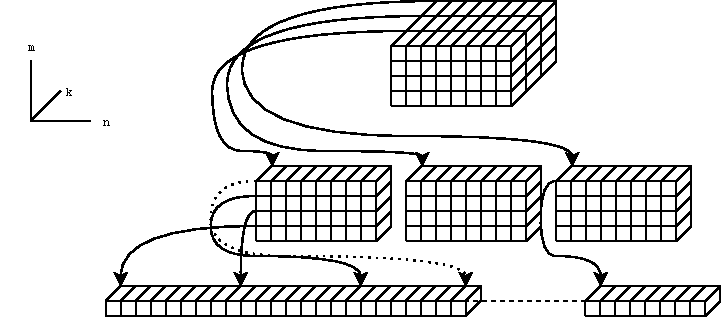
\includegraphics[scale=1.4, angle=270]{chapters/figs/jaggedtoflat.pdf}
  \caption{Flattening a three dimensional jagged array into one flat contiguous
    array.}
  \label{fig:jaggedtoflat}
\end{figure}

\subsection{Analysis of FlattenArray}
The simple algorithm for this flattening is described in pseudocode in figure
\ref{fig:flattenarray}. The implemented algorithm is slightly more complex, as
it has perform various type castings, and also checks for invalid arrays such as
irregular arrays.
In the example, the type $'b$ denotes a primitive type such as booleans or
integers. Type $a$ on the other hand, is any type variable \-- namely array
types.

\begin{figure}[h]
  \centering
\begin{minted}[linenos]{text}
FlattenArray (array : Array of a) : (Array of 'b * Array of int) =
  match typeOf(array) with
  | Array of 'b ->
    return (array, [len(array)])
  | Array of _ ->
    subarrays_and_lengths = map FlattenArray array
    (subarrays, subarrays_lengths) = unzip subarrays_and_lengths
    subarray_lengths = head(subarrays_lengths)
    concatenated_subarrays = concat subarrays
    this_length = len(array)
    lengths = [this_length] @ subarray_lengths
    return (contatenated_arrays, lengths)
\end{minted}
  \caption{Flattening jagged arrays, pseudocode}
  \label{fig:flattenarray}
\end{figure}

When FlattenArray first is called with a jagged array as input, we don't know
how many dimensions this array has. Therefore, we recursively call FlattenArray
on the subarrays of the arrays, until these recursive calls reach a base case.
The base case is the array that does not contain array references, but primitive
values.

\begin{description}
\item[\texttt{L2}]: For a one dimensional jagged array, this branch is taken once.
  For a jagged array of $d$ dimensions, it's taken
  $\prod_{n=1}^{d-1}(\text{subarrays at }d_n)$ times.

\item[\texttt{L3}] is the base case, which takes $O(1)$ time. This is because we
are just returning a tuple with the original array, and singleton array that holds the length of the
array (creating the singleton array is also $O(1).$)

\item[\texttt{L4}]:
  For a jagged array of $d$ dimensions, this branch is taken
  $\prod_{n=1}^{d-1}(\text{subarrays at }d_n)$ times.

\item[\texttt{L5}] is the start of the recursive case. This line is called
  $O(d)$ times, $d$ being the number of dimensions in the jagged array.
  The result of \texttt{map FlattenArray array} is an array of \texttt{a} array references
  and integer array references.

\item[\texttt{L6}] MORE HERE
\item[\texttt{L7}] simply retrieves a reference to the first array in the array
  of subarray lengths. This is $O(1)$.
\item[\texttt{L8}] is by far the most costly line in the function.
  \fsharp{}s \texttt{Array.concat} function takes a sequence of arrays,
  allocates a new array, and copies each element of the old arrays into the new array.
  Each of the $n$ elements in the jagged array is copied to a new array a maximum of $d$
  times, which means we are performing $O(n*d)$ reads and writes.
  
\item[\texttt{L9}] retrieves the length of an array, and is $O(1)$.

\item[\texttt{L10}] appends a singleton array to the accumulated array of
  subarray dimensions, by first creating a singleton array, and then copy both
  the single element and the contents of the accumulated array to a third array
  of their collected length.
\end{description}

All in all, the upper bound on the \texttt{FlattenArray} algorithm is $O(n*d)$.
This is a far cry from the performance of flattening in Futhark. Flattening is
done in $O(1)$, as flattening merely calculates the product of the dimensions of
the array, and returns the result as the new single dimension of the array.

\subsection{Analysis of UnflattenArray}
The algorithm \texttt{UnflattenArray} in figure \ref{fig:unflattenarray}
restores the flat array from the Futhark \csharp{} program, to a jagged array in \fsharp{}.

\begin{figure}[H]
  \centering
\begin{minted}[linenos]{text}
UnflattenArray (lengths : Array of int) (data : Array of a) =
  match len(lengths) with
  | 1 ->
    return data
  | _ ->
    length = head(lengths)
    lengths' = tail(lengths)
    data' = chunk_array length data 
    data'' = map (UnflattenArray lengths') data'
    return data''
\end{minted}
  \caption{Recreating a jagged array from flat array with dimensions}
  \label{fig:unflattenarray}
\end{figure}

Like in \texttt{FlattenArray}, the most expensive line in the function is the
array-manipulating one. In \texttt{UnflattenArray}, it is line 7: For each
dimension in the lengths array, we chunk our data array into multiple smaller
arrays. Each of the $n$ elements in the initial array is moved to a new and smaller array
$d$ times, which makes the complexity of this algorithm $O(n*d)$.

\subsection{Why UnflattenArray hinders a specific tuple type}
\label{subsec:hinderedtupletype}

When an \fshark{} function is invoked, it's arguments are prepared by an
argument converter first. For scalar arguments, the argument is simply returned.
But for array arguments, we must flatten the jagged array into a tuple that
follows Futhark's array representation.

When the Futhark function returns, we then have to unflatten the Futhark arrays
back into jagged arrays. To do this, we naively look at all the values
returned by the Futhark function, and whenever we encounter a tuple of type
\texttt{('a [] * int64 [])}, we assume that this is a flat array that needs to
be unflattened.
This procedure works fine, but has one side effect: \fshark{} doesn't support
entry functions that has (\texttt{('a [] * int64 [])}) tuples in their return
types, because this type is reserved.

To circumvent this, the user is instead encouraged to return the tuple as two
separate values.

\subsection{An alternative solution (FSharkArrays)}
Instead of using jagged arrays (or even multidimensional arrays), we initially
considered implimenting an \fshark{} specific array type, which could be directly
translated to Futhark's flat array structure.

This data type is shown in figure \ref{fig:fsharkarrays0}.
An {\tt FSharkArray<'a>} contains a flat array of {\tt <'a>}, and a list of integers
denoting the lengths of the arrays contained in the flat array.

\begin{figure}[H]
  \centering
\begin{minted}{fsharp}
type FSharkArray<'a> = class
  val mutable flatArray : 'a array 
  val mutable dimensions : int array
  end
\end{minted}
  \caption{The basic structure of an FSharkArray}
  \label{fig:fsharkarrays0}
\end{figure}

This would allow us to skip the flattening and unflattening algorithms that are
currently used for invoking imported Futhark functions, and instead just pass
the contents of the arrays \textit{as is}.

However, this approach was deemed impractical for several reasons.
Jagged arrays readily support getting subarrays and elements using the array
indexing operator intuitively. for example, for a two-dimensional array \texttt{xss :
  int [][]}, we can expect that \texttt{xss.[1]} returns a subarray, and that \texttt{xss.[1].[4]}
returns an integer. 
For example, to get the same functionality for \texttt{FSharkArrays}, we would have to implement the
array operator for \texttt{FSharkArrays} manually. The array operator would have
to access the flat array by calculating an offset using the array operator
operands together with the lengths stored in the \texttt{dimensions} integer
array.

Besides calculating array indexes manually, we would also have to handle that
the index operator must be able to return either an element of some type
\texttt{'a}, or another \texttt{FSharkArray}. This could be handled by
implementing \texttt{FSharkArray} as a discriminated union type instead; as
shown in figure \ref{fig:fsharkarrays1}.

\begin{figure}[H]
  \centering
\begin{minted}{fsharp}
type FSharkArray 'a = FlatArray of ('a array * int array)
                    | Element of 'a
\end{minted}
  \caption{FSharkArray as a discriminated union type}
  \label{fig:fsharkarrays1}
\end{figure}
This way, an \texttt{FSharkArray} can be either an array or an element. However,
we then have a third problem.
Wherever we are using \texttt{FSharkArray 'a}, our elements from the arrays will be wrapped as
\texttt{Element of 'a}s.

This means that we will have to either implement a custom set of \fsharp{}
operators and standard library functions which unwraps \texttt{Elements} before
passing them on to the actual operator or function, or at least implement an
unwrapper function of type $unwrap : Element~of~'a~\to~'a$, which must be applied
everywhere in functions that uses both \texttt{FSharkArrays} and \fsharp{}
standard library functions.

\subsection{Conclusion on arrays}
Ultimately, choosing between jagged arrays, multidimensional arrays and
FSharkArrays became a question of simplicity vs. performance.
For \fshark{}, I had the liberty to focus solely on simplicity, as \fshark{}
code is neither intended or even efficient when executed as native FSharp code.
Therefore I could choose to let \fshark{} use jagged arrays, instead of any of
the other options.

The syntax for declaring a jagged array type closely
resembles Futhark's multidimensional array syntax (take for instance FSharp's
\texttt{int[][]} versus Futhark's \texttt{[][]i32} for declaring
two-dimensional integer arrays).
The close similarities between Futhark and \fshark{} code means that \fshark{}
generated Futhark code is easier to read for debugging purposes, and likewise
makes Futhark code easier to port to \fshark{}.

%%% Local Variables:
%%% mode: latex
%%% TeX-master: "../thesis"
%%% End:

\chapter{The \fshark{} Compiler and Wrapper}
\section*{Introduction}
\label{sec:fsharkcompiler}
Parsing and building a regular F\# program is trivial when using official build tools like
\texttt{msbuild} or \texttt{fsharpc}.
But in the case of \fshark{}, we are not interested in the final result from the
F\# compiler, but merely its half-finished product.

As the F\# Software Foundation offers the official F\# Compiler as a freely
available NuGet package for F\# projects, we can use this package
\texttt{FSharp.Compiler.Services} to parse the entire input \fshark{} program and
give us a Typed Abstract Syntax Tree of the FSharp expressions therein.

The F\# Software Foundation actively encourages developers to create projects
using the F\# compiler library, they have published the collected F\# compiler
as a NuGet package, alongside a tutorial\ref{fsharptutorial}on the usage of the
various compiler parts.

For \fshark{}, the Compiler Services package is used to compile a Typed Abstract
Syntax Tree from a wellformed \fshark{} source code file, which we then
convert into- and print as a valid Futhark program.
The Typed Abstract Syntax Tree is merely an AST that already has tagged all the
contained expressions with their respective types.

We'll start with a detailed explanation of the \fshark{} Compiler Pipeline.

\subsection*{The \fshark{} Compiler Pipeline in practice}
To examine the compiler pipeline in action, we'll go through the motions with
the small example program displayed in figure \ref{fig:fsharkusageexample}.

\begin{figure}[h]
  \centering
    \begin{minted}[linenos,breaklines]{fsharp}
module FSharkExample
open FShark.Main

[<EntryPoint>]
let main argv =
  let wrapper = 
    new FSharkWrapper(
      libName="ExampleModule",
      tmpRoot="/home/mikkel/FShark",
      preludePath= "/home/mikkel/Documents/fshark/FSharkPrelude/bin/Debug/FSharkPrelude.dll",
      openCL=true,
      unsafe=true,
      debug=false
      )
  wrapper.AddSourceFile "../../srcs/ExampleModule.fs"
  wrapper.CompileAndLoad
  let xs = [|1;2;3;4|]
  let input = [|xs|] : obj array
  let xs' = wrapper.InvokeFunction "MapPlusTwo" input :?> int array
  printfn "Mapping (+2) over %A gives us %A" xs xs'
  0
    \end{minted}
  \caption{An F\# program using \fshark{}}
  \label{fig:fsharkusageexample}
\end{figure}

We begin by constructing an instance of the \fshark{}Wrapper. It has the following
mandatory arguments:

\begin{description}
\item[\texttt{libName}]\hfill\\
  This is the library name for the \fshark{} program. In the final Futhark
  \texttt{.cs} and \texttt{.dll} files, the main class will have the same name
  as the \texttt{libName}. This doesn't really matter if \fshark{} is just used
  as a JIT compiler, but it's good to have a proper name if the user only wants
  to use the compiler parts of \fshark{}.

\item[\texttt{tmpRoot}]\hfill\\
  The \fshark{} compiler works in its own temporary directory. This argument must
  point to a directory where F\# can write files and execute subprocesses
  (Futhark- and C\# compilers) which also has to write files.
  
\item[\texttt{preludePath}]\hfill\\
  The \fshark{} compiler needs the FShark prelude available to compile FShark
  programs. 

\item[\texttt{openCL}]\hfill\\
  Although Futhark (and therefore \fshark{}) is most effective on OpenCL-enabled
  computers, the benchmarks in \ref{sec:benchmarks} still show a significant
  speed increase for non-OpenCL Futhark over native F\# code.
  Therefore, \fshark{} is also available for non-OpenCL users. Use this flag to
  tell \fshark{} whether Futhark should compile C\# with or without OpenCL.
  
\item[\texttt{unsafe}]\hfill\\
  For some Futhark programs, the Futhark compiler itself is unable to tell
  whether certain array operations or SOAC usages are safe, and will stop the
  compilation, even though the code should (and does) indeed work.
  To enable these unsafe operations, pass a \texttt{true} flag to the compiler.

\item[\texttt{debug}]\hfill\\
  Passing the debug flag to the \fshark{} compiler enables various runtime
  debugging features, for instance benchmarking the time it takes to run various
  parts of the compiler.
\end{description}

Now, we can pass a source file to the \fshark{} wrapper, compile\footnote{See
  subsection \ref{subsec:fsharkwrappercompiles}} it and load it into the \fshark{} wrapper object.

To use the compiled \fshark{} function, we must first wrap our designated input in
an \texttt{obj array}. In this case, our chosen \fshark{} function takes one
argument, an \texttt{int array}. We define this array, and construct an argument
array containing this single element. If the \fshark{} function takes two
arguments, we define an input \texttt{obj array} with two elements, and so
forth.
It is important to declare the input array as an \texttt{obj array}. Otherwise,
F\#s own type checker might very well faultily infer the input array as
something else. In this particular case, \texttt{input} would've been inferred
as being an \texttt{int array array}, until we declared its type specifically.

We then invoke the desired function through the wrapper. As all
reflection-invoked functions return a value of type \texttt{obj}, we need to
downcast this object manually.
In this example, we use F\#s downcast operator \texttt{(:?>)} to declare the
return value as an \texttt{int array}. The actual return type is always the same as the
return type declared in the source \fshark{} file.

\subsection*{When \fshark{} Wrapper Compiles}
\label{sec:fsharkwrappercompiles}
The general way to compile and load an \fshark{} program into the FShark Wrapper,
is by adding \fshark{} source files to the wrapper object by calling the
\texttt{AddSourceFile} method, and followingly calling the \texttt{CompileAndLoad}
method. Although the \fshark{} wrapper also offers other methods of loading and
compilation, this is the primary one, as it initiates the entire \fshark{}
compilation pipeline.

\begin{figure}[h]
  \centering
  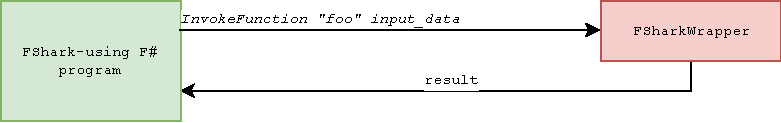
\includegraphics{chapters/figs/csharp/pipeline_step_3.pdf}
  \caption{The \fshark{} compilation pipeline}
  \label{fig:fsharkcompilerpipeline}
\end{figure}


When calling \texttt{CompileAndLoad}, the supplied \fshark{} source files are
concatenated into one long source file, and written to a temporary location.
An FSharpChecker is then initialized, so we can parse and type check the
concatenated source code. The FSharpChecker is a class exported by the FSharp
Compiler Services, and is a class that lets developers use part of the F\#
compilation pipeline at runtime.

We supply the FSharpChecker with the path to our precompiled \fshark{}Prelude
assembly, and then call its \texttt{ParseAndCheckProject} method on to receive
an assembly value, which contains the complete Typed Abstract Syntax Tree of our
\fshark{} program, in the form of an \texttt{FSharpImplementationFileDeclaration}.

If the \fshark{} developer followed the guidelines to write a well-formed FShark
module, the main declaration of the program, the
\texttt{FSharpImplementationFileDeclaration}, should contain a single
\texttt{FSharpEntity}, which in turn contains all the remaining declarations in
the program.

\subsubsection*{The declaration types within F\#'s Typed AST}
The \texttt{FSharpImplementationFileDeclaration} type has three union cases.
\begin{description}
\item[\texttt{InitAction of FSharpExpr}] \hfill\\
  \texttt{InitAction}s are \fsharpexpr{}s that are executed at the
  initialization of the containing entity. These are not supported in \fshark{}.

\item[\texttt{Entity of FSharpEntity * FSharpImplementationFileDeclaration list}]\hfill\\
  An \texttt{Entity} is the declaration of a type or a module. In the case of
  \fshark{}, three different kinds of entities are supported:
  \begin{description}
  \item[FSharpRecords] are standard record types, and can be translated to
    Futhark records with ease.
    This entity has an empty \texttt{FSharpImplementationFileDeclaration list}.
  \item[FSharpAbbreviations] are type abbreviations, and are easily translated
    into Futhark type aliases.
    This entity has an empty \texttt{FSharpImplementationFileDeclaration list}.
  \item[FSharpModules] are named modules which contains subdeclarations.
    In this case, we retrieve the subdeclarations from the \texttt{FSharpImplementationFileDeclaration list}.
    The \fshark{} compiler supports building FShark modules, but current
    limitations demands that modules are flattened when compiled to Futhark.
    This also means that function name prefixes in function calls are stripped
    when compiled to Futhark.
  \end{description}
\item[\texttt{MemberOrFunctionOrValue of \\ FSharpMemberOrFunctionOrValue *
    FSharpMemberOrFunctionOrValue list list * FSharpExpr}]\hfill\\
  F\# doesn't differ between functions and values, which means that a function
  is merely a value with arguments.
  A pattern matched \texttt{MemberOrFunctionOrValue} value has the form
  \texttt{MemberOrFunctionOrValue (v, args, exp)}, where \texttt{v} contains the
  name and the type of the variable.
  If the \texttt{args} list is empty, \texttt{v} is simply a variable. If not,
  \texttt{v} is a function. \texttt{exp} contains the \fsharpexpr{} that
  \texttt{v} is bound to. An \fsharpexpr{} can be anything from a numeric
  constant to a very long function body.
\end{description}

In figure \ref{fig:validfsharkprogram} we see a small but valid \fshark{} program. It
reads like a regular F\# program, but contains the three vital parts that makes
it usable as an \fshark{} program.

\begin{figure}[h]
  \centering
  \begin{minted}[xleftmargin=5pt,linenos]{fsharp}
    module ExampleModule
    open FSharkPrelude

    module SomeValues =
      let Four : int = 4

      let SomePlus (x : int) (y : int) : int = x + y

    [<FSharkEntry>]
    let TimesTwo (x : int) : int =
      SomeValues.SomePlus x x
  
    [<FSharkEntry>]
    let MapPlusTwo (xs : int array) : int array =
      Map ((+)2) xs

    let PlusSeven (x : int) : int =
      SomeValues.SomePlus x 7
  \end{minted}
  \caption{A valid \fshark{} program}
  \label{fig:validfsharkprogram}
\end{figure}

\begin{itemize}
\item The module declaration on the first line declares that the following code
  is inside a module. In this case, we are declaring the module
  \texttt{ExampleModule}, although we could use any valid F\# module name.
  As shown in figure \ref{fig:validfsharkprogramresult}, the top module
  declaration falls away during compilation, so only the top module contents are
  left.

\item This \texttt{open} statement ensures that the F\# Compiler Services has
  access to the \fshark{}Prelude during the compilation. It is possible to write an
  \fshark{} program which doesn't use the FSharkPrelude, but this removes access to
  the SOACs that we use to write our data parallel programs.

\item The \texttt{[<\fshark{}Entry>]} attributed function \texttt{TimesTwo} ensures
  that the resulting Futhark library from the \fshark{} compiler has at least one
  entry point function.
  Without any entry point functions, we won't have any functions in the final
  compiled \fshark{} program.
\end{itemize}

\begin{figure}
  \centering
\begin{lstlisting}[language=Futhark]
    let Four : i32 = 4i32
    let SomePlus (x : i32) (y : i32) : i32 =
      ((x i32.+ y))
    entry TimesTwo (x : i32) : i32 =
      unsafe SomePlus(x) (x)
    entry MapPlusTwo (xs : []i32) : []i32 =
      unsafe map (let x = 2i32 in
                  (\(y : i32) -> ((x i32.+ y)))) (xs)
    let PlusSeven (x : i32) : i32 =
      SomePlus(x) (7i32)
      \end{lstlisting}
  \caption{A valid \fshark{} program, compiled to Futhark}
  \label{fig:validfsharkprogramresult}
\end{figure}

In figure \ref{fig:validfsharkprogramresult} we see the resulting Futhark program.
For now, we will ignore the transformations that have happened, except for two
things: The \texttt{Map} function (called from \fshark{}Prelude) has been rewritten
as the plain Futhark SOAC \texttt{map} in lowercase, and the module SomeValues has been
flattened (see sec \ref{futurework:modules} for future plans.)

This Futhark program is then stored in a temporary location in the user's file
system, and compiled into as a library, using Futhark's C\# compiler, either
with or without OpenCL support. Finally after this compilation, we can invoke
the resulting .dll file from within the \fshark{}-using F\# program.

\subsection*{Building \fshark{} from the Typed AST}
\label{sec:fsharkcompilerrules}
Only the supported FSharpExpr's has been listed here, but the full range of
FSharpExpr's are available on \cite{typedtree}.

\subsection*{FSharp-to-\fshark{}IL rules}
INTRODUCTION HERE

For these translations, we will disregard that all \fsharpexpr{}s are union
cases of the F\# data type \texttt{BasicPatterns}.


\begin{figure}
  \begin{framed}
    
  \centering
\begin{tabular}{@{}l c l}% to \linewidth {l c X}
  $\evals{Entity(\lit{IsFSharpRecord}, [(field_0 : \tau_0), \ldots, (field_n : \tau_n)])}$ & & \\
  $= \lit{FSharkRecord([}(field_0 : \evals{\tau_0}), \ldots, (field_n : \evals{\tau_n})\lit{])}$ & & \\
  ~ \\
\end{tabular}
\begin{tabular}{@{}l c l}% to \linewidth {l c X}
  $\evals{Entity(\lit{IsFSharpTypeAbbreviation}, alias, \tau)}$ & & \\
  $= \lit{FSharkTypeAlias(} alias, \evals{\tau}\lit{)}$ & & \\
  ~ \\
\end{tabular}
\begin{tabular}{@{}l c l}% to \linewidth {l c X}
  $\evals{Entity(\lit{IsFSharpModule}, [decl_0,\ldots,decl_n])}$ & & \\
  $= [\evals{decl_0},\ldots,\evals{decl_n}]$ & & \\
  ~ \\
\end{tabular}
\begin{tabular}{@{}l c l}% to \linewidth {l c X}
  $\evals{MemberOrFunctionOrValue((name, \tau^{*}, IsEntryFunction), [(arg_0 : \tau_0), \ldots, (arg_n : \tau_n)], e)}$ & & \\
  $= FSharkVal(IsEntryFunction, \lit{FSharkFunction}([\evals{\tau_0}, \ldots, \evals{\tau_n}], \evals{\tau^{*}}),name, [arg_0,..,arg_n],\evals{e})$ & & \\
  ~ \\
\end{tabular}
\caption{Rules for translating FSharp declarations to FShark
    declarations}
  \end{framed}

\end{figure}


\begin{figure}
  \centering
\begin{tabular}{@{}l c l}% to \linewidth {l c X}
  $\evals{System.Int8}$ & $=$ & $\lit{FInt8} $ \\ 
  $\evals{System.Int16}$ & $=$ & $\lit{FInt16}$
  \\
  $\evals{System.Int32}$ & $=$ & $\lit{FInt32} $ \\ 
  $\evals{System.Int64}$ & $=$ & $\lit{FInt64} $
  \\
  $\evals{System.UInt8}$ & $=$ & $\lit{FUInt8} $ \\ 
  $\evals{System.UInt16}$ & $=$ & $\lit{FUInt16} $ 
  \\
  $\evals{System.UInt32}$ & $=$ & $\lit{FUInt32} $ \\ 
  $\evals{System.UInt64}$ & $=$ & $\lit{FUInt64} $ 
  \\
  $\evals{System.Single}$ & $=$ & $\lit{FSingle} $ \\ 
  $\evals{System.Double}$ & $=$ & $\lit{FDouble} $ 
  \\
  $\evals{System.Boolean}$ & $=$ & $\lit{Bool} $ \\ 
  $\evals{System.Array~\tau}$ & $=$ & $\lit{\fshark{}Array }\evals{\tau}$
  \\
  $\evals{System.Tuple~(\tau_0 \times \ldots \times \tau_n)}$ & $=$ & $\lit{\fshark{}Tuple}~(\evals{\tau_0}~\times~\ldots~\times~\evals{\tau_n)}$ \\ ~ \\
\end{tabular}

INSERT NOTE ON RULE FOR TUPLE ('a [] * long [])

\caption{Rules for translating .NET types to FSharkIL types}
\end{figure}

\begin{figure}
  \centering
\begin{tabular}{@{}l c l}% to \linewidth {l c X}
  $\evals{\lit{FInt8}}}$ & $=$ & $\lit{i8} $ \\ 
  $\evals{\lit{FInt16}}$ & $=$ & $\lit{i16}$
  \\              
  $\evals{\lit{FInt32}}$ & $=$ & $\lit{i32} $ \\ 
  $\evals{\lit{FInt64}}$ & $=$ & $\lit{i64} $
  \\
  $\evals{\lit{FUInt8}}$ & $=$ & $\lit{u8} $ \\ 
  $\evals{\lit{FUInt16}}$ & $=$ & $\lit{u16} $ 
  \\               
  $\evals{\lit{FUInt32}}$ & $=$ & $\lit{u32} $ \\ 
  $\evals{\lit{FUInt64}}$ & $=$ & $\lit{u64} $ 
  \\
  $\evals{\lit{FSingle}}$ & $=$ & $\lit{f32} $ \\ 
  $\evals{\lit{FDouble}}$ & $=$ & $\lit{f64} $ \\
  $\evals{\lit{Bool}}$ & $=$ & $\lit{bool} $ \\ 
  $\evals{\lit{FSharkArray}~\tau}$ & $=$ & $\lit{[]}\evals{\tau}$
  \\
  $\evals{\lit{\fshark{}Tuple}~({\tau_0}~\times~\ldots~\times~{\tau_n})}$ & $=$ & $(\evals{\tau_0},\ldots,\evals{\tau_n})$ \\ ~ \\
\end{tabular}
\caption{\texttt{\fshark{}IL} types to Futhark types}
\end{figure}

\begin{figure}
  \centering
  \begin{tabular}{@{}l c l}% to \linewidth {l c X}
  $\evals{Const(obj, \tau)}$ & $=$ & $\lit{Const(}obj, \evals{\tau} \lit{)}$ \\
  $\evals{Value(v)}$ & $=$ & $\lit{Var(}v{)}$ \\
  $\evals{AddressOf(v)}$ & $=$ & $\evals{v}$ \\
  $\evals{NewTuple(\_, [e_0,...,e_1])}$ & $=$ & $\lit{Tuple([}\evals{e_0},\ldots, \evals{e_n}\lit{])}$ \\
  $\evals{NewRecord((v_0 : \tau_0 * \ldots * v_n : \tau_n), [e_0,...,e_1])}$ & $=$ & $\lit{Record([}(v_0,\evals{e_0}),\ldots,(v_n,\evals{e_n})\lit{])}$ \\
  $\evals{NewArray(\tau, [e_0,...,e_1])}$ & $=$ & $\lit{List(}\evals{\tau},\lit{[}\evals{e_0},\ldots, \evals{e_n}\lit{]}\lit{)}$ \\
  $\evals{TupleGet(\_, i, e)}$ & $=$ & $\lit{TupleGet(}\evals{e}, i{)}$ \\
  $\evals{FSharpFieldGet(e, \_, field)}$ & $=$ & $\lit{RecordGet(}field, \evals{e}{)}$ \\
    $\evals{Call(\_, \lit{GetArray}, \_, nil, [e_0, e_1])}$ & $=$ & $\lit{ArrayIndex(}\evals{e_0},\evals{e_1}]\lit{)}$ \\
    $\evals{Call(\_, name, \_, nil, [e_0, \ldots, e_n])}$ & $=$ & $\lit{Call(}name, [\evals{e_0},\ldots,\evals{e_n}]\lit{)}$ \\
    $\evals{Call(\_, name, \_, \tau, [e_0, \ldots, e_n])}$ & $=$ & $\lit{TypedCall(}\evals{\tau},name, [\evals{e_0}, \ldots, \evals{e_n}]\lit{)}$ \\
    $\evals{Call(\_, infixOp, \_, \tau, [e_0, e_1])}$ & $=$ & $\lit{InfixOp(}infixOp, \evals{\tau}, \evals{e_0}, \evals{e_1}\lit{)}$ \\
    $\evals{Call(\_, unaryOp, \_, \tau, [e_0])}$ & $=$ & $\lit{UnaryOp(}unaryOp, \evals{\tau}, \evals{e_0}\lit{)}$ \\
  $\evals{Let(v, e_0, e_1)}$ & $=$ & $\lit{LetIn(}v, \evals{e_0}, \evals{e_1}\lit{)}$ \\
  $\evals{IfThenElse(e_0, e_1, e_2)}$ & $=$ & $\lit{If(}\evals{e_0}, \evals{e_1}, \evals{e_2}\lit{)}$ \\
  $\evals{Lambda((v : \tau), e)}$ & $=$ & $\lit{Lambda(}v, \evals{\tau}, \evals{e} \lit{)}$ \\
  $\evals{Application(func, \_, [e_0, \ldots, e_n])}$ & $=$ & $\lit{Application(}\evals{func}, \lit{[}\evals{e_0},\ldots, \evals{e_n}\lit{])}$ \\
  $\evals{TypeLambda(e)}$ & $=$ & $\evals{e}$ \\
  $\evals{DecisionTree(\_, \_)}$ & $=$ & $\lit{Pass}$ \\
  $\evals{DecisionTreeSuccess(\_, \_)}$ & $=$ & $\lit{Pass}$ \\ ~ \\
\end{tabular}
\caption{Translation rules for FSharp expressions to FSharkIL expressions}
\end{figure}

  
\begin{figure}
  \centering
  \begin{tabular}{@{}l c l}% to \linewidth {l c X}
  $\evals{Const(obj, \tau )}$ & $=$ & $obj\evals{\tau}$ \\
  $\evals{Var(v)}$ & $=$ & $v$\\
  $\evals{Tuple([e_0,\ldots, e_n])}$ & $=$ & $(\evals{e_0},\ldots, \evals{e_n})$\\
  $\evals{Record([(v_0, e_0),\ldots,(v_n,e_n)])}$ & $=$ & $\{v_0=\evals{e_0},~\ldots,~v_n=\evals{e_n}\}$ \\
  $\evals{List(}\evals{\tau},\lit{[}\evals{e_0},\ldots, \evals{e_n}\lit{]}\lit{)}$ & $=$ & $[\evals{e_0},~\ldots,~\evals{e_n}]$\\
  $\evals{TupleGet(}\evals{e}, i{)}$ & $=$ & $\evals{e}.i$ \\
  $\evals{RecordGet(field, e)}$ & $=$ & $\evals{e}.field$ \\
  $\evals{ArrayIndex(e_{arr},[e_0, \ldots, e_n])}$ & $=$ & $\evals{e_{arr}}\lit{[}\evals{e_0},\ldots,\evals{e_n}\lit{]}$ \\
    
  $\evals{Call(name, [e_0,\ldots,e_n]\lit{)}}$ & $=$ & $name~(\evals{e_0})~\ldots~(\evals{e_n})$ \\
  $\evals{TypedCall(}\evals{\tau},name, [\evals{e_0}, \ldots, \evals{e_n}]\lit{)}$ & $=$ & $\evals{\tau}.name~(\evals{e_0})~\ldots~(\evals{e_n})$ \\
  $\evals{InfixOp(}infixOp, \evals{\tau}, \evals{e_0}, \evals{e_1}\lit{)}$ & $=$ & $(\evals{e_0})~\evals{\tau}.infixOp~(\evals{e_1})$ \\
  $\evals{UnaryOp(}unaryOp, \evals{\tau}, \evals{e_0}\lit{)}$ & $=$ & $\evals{\tau}.unaryOp~(\evals{e_0})$ \\

  $\evals{LetIn(}v, \evals{e_0}, \evals{e_1}\lit{)}$ & $=$ & $\mathtt{let}~v~=~\evals{e_0}~\mathtt{in}~\evals{e_1}$ \\

  $\evals{If(}\evals{e_0}, \evals{e_1}, \evals{e_2}\lit{)}$ & $=$ & $\mathtt{if}~\evals{e_0}~\mathtt{then}~\evals{e_1}~\mathtt{else}~\evals{e_2}$ \\

  $\evals{Lambda(v, \evals{\tau}, \evals{e} \lit{)}}$ & $=$ & $\mathtt{\backslash}(v : \evals{\tau})~\mathtt{->}~\evals{e}$ \\
  $\evals{Application(\evals{func}, \lit{[}\evals{e_0},\ldots, \evals{e_n}\lit{])}}$ & $=$ & $(\evals{func})~(\evals{e_0})~\ldots~(\evals{e_n})$ \\
  $\evals{Pass}$ & $=$ & $\epsilon$ $$ \\
\end{tabular}
\caption{\texttt{FSharkIL} expressions to Futhark}
\end{figure}

\section{Design choices in writing the FShark Compiler}
% should I write parser manually or just use FSharp library
% this meant a design process where I disected F# programs using Riders debugger

% biggest hurdle for compiler: updated Futhark lang specifications: 

% what could be expanded?
% maybe make a loop function that imitates the futhark loop construct

%%% Local Variables:
%%% mode: latex
%%% TeX-master: "../thesis"
%%% End:
\chapter{The Futhark \csharp{} backend}
In this chapter we first demonstrate how we want to use Futhark-generated
\csharp{} GPU libraries in \csharp{} programs. We then describe the architecture
needed for compiling such \csharp{} libraries using the Futhark compiler, and
what features we need in our code generator to successfully generate standalone
\csharp{} programs embedded Futhark-generated GPU kernels. 
We then show the finished design of the generated Futhark \csharp{} code, and
describe the segments in the code segment by segment.

We discuss choices taken for memory management in Futhark \csharp{} programs,
and compare different methods of memory management by their runtime performance.

Finally, we discuss how and why the OpenCL library ``\texttt{Cloo}'' was chosen
as a backend for Futhark's \csharp{} compiler.

\section{Recap on using Futhark \csharp{} libraries}
For a given Futhark program (such as the one shown in figure \ref{fig:shortfutharkprogram3'}), 
we want to be able to compile the program to a
\csharp{} library from the command line like shown in figure \ref{fig:shortfutharkprogram4'}.
This results in a compiled \csharp{} dynamically linked library\footnote{A
  \texttt{.dll} file}.
Then, we can include this library in a \csharp{} project like any other external
library, and use its functions as expected, like shown in figure \ref{fig:shortfutharkprogram5'}.

\begin{figure}[H]
\begin{subfigure}
  \centering
  \begin{lstlisting}[language=Futhark]
entry mapPlus2 (xs : []i32) : []i32 =
  map (+2) xs
  \end{lstlisting}
  \caption{A short Futhark program called mapPlus2.fut}
  \label{fig:shortfutharkprogram3'}
\end{subfigure}

\begin{subfigure}
  \centering
  \begin{lstlisting}[language=sh]
$ futhark-cs --library -o MapPlus2.dll mapPlus2.fut
  \end{lstlisting}
  \caption{We call the Futhark-to-\csharp{} compiler \texttt{futhark-cs} on
    mapPlus2.fut}
  \label{fig:shortfutharkprogram4'}
\end{subfigure}

\begin{subfigure}
  \centering
\begin{minted}[linenos]{csharp}
using System.Linq;
using MapPlus2;

public class Program
{
    public static int Main(string[] args)
    {
        var mapplus2Class = new MapPlus2();
        var xs = Enumerable.Range(0, 1000000).ToArray();
        var xs_result = mapplus2Class.mapPlus2(xs)
    }
}
\end{minted}
  \caption{We use the compiled Futhark program as any other library.}
  \label{fig:shortfutharkprogram5'}
\end{subfigure}
\end{figure}

\subsection{Compiling and using Futhark \csharp{} executables}
\label{subsec:futharkcsexe}
Not all users are interested in using Futhark programs as parts in other code
projects. Instead, these users can opt to compile Futhark programs into
executables. Recalling the Futhark example in
\Cref{fig:shortfutharkprogram3',fig:shortfutharkprogram4',fig:shortfutharkprogram5'},
we instead opt to compile the Futhark program as an executable program.

Keeping the Futhark source file \texttt{mapPlus2.fut} from
\ref{fig:shortfutharkprogram3'}, we use futhark-cs to compile the program into
an executable; the command line is shown below: %in figure \ref{fig:shortfutharkprogram4''}.
  \begin{lstlisting}[language=sh]
$ futhark-cs -o MapPlus2 mapPlus2.fut
  \end{lstlisting}
%
Here, the compiler produces an executable named \texttt{MapPlus2} from the
original source file, named {\tt mapPlus2.fut}.

We can now execute this program in one of two ways.
The first way is to write our arguments in a string in the command line, and
to \texttt{echo} them through a pipe into the executable, as shown below:
  \begin{lstlisting}[language=sh]
$ echo "[1,2,3,4,5,6,7]" | ./MapPlus2
[3i32, 4i32, 5i32, 6i32, 7i32, 8i32, 9i32]
  \end{lstlisting}
%This method is shown in figure \ref{fig:shortfutharkprogram5''}. 
Here, the one argument we are using is 
an integer array. We pass the array to the executable, and it prints the result
to \texttt{stdout} after it has finished. The \texttt{i32}'s tells us that the
result array holds 32 bit signed integers.
For multi-argument entry functions, we separate the arguments with whitespace.

For the second method, we store our arguments in a dataset file. For example, we
can store our integer array in a plain text file, named {\tt array.in}, 
as shown below: %shown in figure \ref{fig:array.in}.
  \begin{lstlisting}
[1,2,3,4,5,6,7]
  \end{lstlisting}
We can then use the command line to redirect the contents of the dataset file
into our command:
%as shown in figure \ref{fig:shortfutharkprogram5'''}.
  \begin{lstlisting}[language=sh]
$ ./MapPlus2 < array.in
[3i32, 4i32, 5i32, 6i32, 7i32, 8i32, 9i32]
  \end{lstlisting}
If we want to, we can redirect the output from stdout to a file of our own
choice: %shown in figure \ref{fig:shortfutharkprogram6'}. 
  \begin{lstlisting}[language=sh]
$ ./MapPlus2 < array.in > result.txt
$ cat result.txt
[3i32, 4i32, 5i32, 6i32, 7i32, 8i32, 9i32]
  \end{lstlisting}
Here, we redirect Futhark's output to \texttt{result.txt}, and print it to 
\texttt{stdout} by using \texttt{cat} to confirm that we have obtained indeed 
the correct result.

\section{The Futhark \csharp{} compiler architecture}
In figure \ref{fig:ccompiler} we showed a rough sketch of the
Futhark compiler's architecture. To sufficiently explore the contribution of
this thesis, we will however first need a more detailed view of the architecture
we need to implement to accomplish our goal.
This architecture is depicted in figure \ref{fig:futharkcompilerlowerlevel}.

\begin{figure}[H]
  \centering
  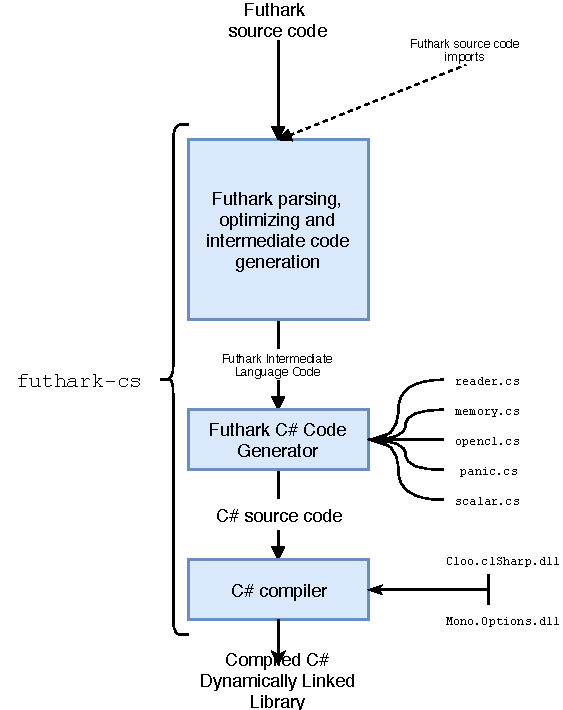
\includegraphics[scale=0.85]{chapters/figs/csharp/futharkcsarchitecture.pdf}
  \caption{The Futhark \csharp{} architecture, including necessary imports.}
  \label{fig:futharkcompilerlowerlevel}
\end{figure}

We will now describe its three main steps:
\begin{description}
\item[Step 1:]\hfill\\
  A Futhark source file is passed to the Futhark compiler (like in figure
  \ref{fig:shortfutharkprogram4'}). Although only the main source file is passed
  as an argument to the compiler, the compiler also includes any imports in the
  main source file, if there should be any.

  This first part of the Futhark compiler is responsible for parsing the passed
  Futhark program, including imports, and performs all type checks, SOAC
  optimizations, fusions and so on~\cite{pldi17}. The result of this process is a
  Futhark program expressed in imperative internal intermediate called \texttt{ImpCode}.
  The \texttt{ImpCode} grammar is included in the appendix. The \texttt{ImpCode}
  language contains everything from memory operations like allocating and
  deallocation memory (both on system memory and on the GPU), interfacing with
  the OpenCL device (like copying buffers back and forth between the system and
  the GPU, setting kernel arguments and launching computation kernels), and also
  basic expressions like addition and multiplication.

\item[Step 2:]\hfill\\
  The \csharp{} code generator takes the Futhark program written in
  \texttt{ImpCode}, and expresses it as \csharp{} source code.
  For example, we can take the simple \texttt{ImpCode} expression in figure \ref{fig:impcode},
  and rewrite it as \csharp{} code, shown in figure \ref{fig:impcodeascs}.
  \begin{figure}[H]
    \centering
\begin{minted}{lisp}
SetScalar "x" (
    BinOpExp Add 
      (ValueExp (IntValue (Int32Value 4))) 
      (ValueExp (IntValue (Int32Value 5)))
    )
\end{minted}
    \caption{Setting int x to 4+5 with simplified \texttt{ImpCode}}
    \label{fig:impcode}
  \end{figure}

\begin{figure}[H]
\centering
\begin{minted}{csharp}
int x = 4 + 5;
\end{minted}
\caption{Setting int x to 4+5 in \csharp{}}
\label{fig:impcodeascs}
  \end{figure}

Besides taking an \texttt{ImpCode} program as input, it also embeds a set of
prewritten \csharp{} libraries\footnote{\texttt{reader.cs} et al} into the generated \csharp{} code. These
libraries are ncessary for the finished \csharp{} program, and are described in
section~\ref{subsec:runtimelibs}.\\
The resulted \csharp{} source code is passed to a \csharp{} compiler, but also
written to disk so it is available for the developer.

\item[Step 3:]\hfill\\
  To use the \csharp{} code, we need to compile it using the command shown in
  figure \ref{fig:callcsc}. We tell the compiler that we have external libraries
  stored at the location stored at \texttt{\$MONO\_PATH}\footnote{An environment
  variable that should be set to a directory containing external runtime
  libraries for Mono runtime usage.}, and we tell the compiler to
  reference two extra external libraries \texttt{Mono.Options.dll} and
  \texttt{Cloo.clSharp.dll}, as we need these libraries in the Futhark \csharp{} programs.

  We also add the library flag ({\tt -lib}) so that \texttt{csc} compiles to a \texttt{.dll} file instead of
  generating an executable. Finally we add the \texttt{/unsafe} flag so the
  compiler allows us to use \texttt{unsafe} statements in the \csharp{} program.

\begin{figure}[H]
  \centering
  \begin{lstlisting}[language=sh]
$ csc -lib:$MONO_PATH -r:Mono.Options.dll \
      -r:Cloo.clSharp.dll /unsafe mapPlus2.cs
  \end{lstlisting}
  \caption{Calling the \csharp{} compiler on the resulted {\tt mapPlus2.cs} file.}
  \label{fig:callcsc}
\end{figure}

However, the last step in \texttt{futhark-cs} does this for the user
automatically, as long as the user has set the required \texttt{\$MONO\_PATH}
variable, and that the directory that \texttt{\$MONO\_PATH} points to, contains the
required libraries.

\end{description}

This thesis leverages the already existent Futhark codebase to implement 
steps 1 and 3, hence does not bring important contributions to them. 
Instead, the contribution of this thesis refers to implementing the 
code generator described in step 2.

%\subsection{Designing the Futhark \csharp{} generator}
In the grand scheme of things, the Futhark \csharp{} generator is not
interesting by itself. The entire contribution to the Futhark compiler is
around 4500 SLOC, split 50/50 between \csharp{} and Haskell code.
In the remaining of this chapter we will instead discuss at a high level
the {\em structure of the generated code}.

%\clearpage

\section{The Structure of the Generated \csharp{} Code}
As previously discussed, Futhark code can be compiled (1) to a library 
that is usable in both \csharp{} and \fsharp{} programs, and (2) also
to a standalone \csharp{} executable, which, for example, takes argument 
inputs from the \texttt{stdin} stream, and prints the
results to \texttt{stdout}.

As this thesis focuses on interoperability, we will primarily concentrate on the
design of the \csharp{} code generated for Futhark libraries, and mention
design differences in the cases in which the Futhark executables differs 
from the translation used for libraries.
Figure \ref{fig:futharkcsclasses} shows a high level representation of the
generated \csharp{} classes for the standalone- and library-compilation cases.

\begin{figure}[h]
  \centering
  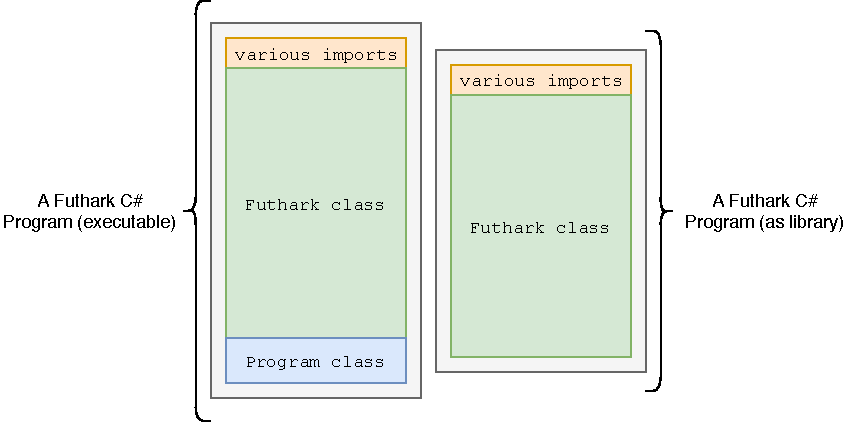
\includegraphics[scale=0.85]{chapters/figs/csharp/futharkcs_wide.pdf}
  \caption{The two possible types Futhark \csharp{} programs}
  \label{fig:futharkcsclasses}
\end{figure}

Here follows a short explanation of the different sections of the Futhark
programs.
\begin{description}
\item[\texttt{various imports}] \hfill \\
  This part consists of \texttt{using} statements that import the
    various libraries on which the translation relies into the \csharp{} program.
  
\item[\texttt{Futhark class}] \hfill \\
  The Futhark class is a singleton class that encapsulates all needed functionality
    for executing the exports (entry-points) defined in the original Futhark file.
  The Futhark class is discussed in subsec \ref{subsec:futharkclass}.
  
\item[\texttt{Entry functions}] \hfill \\
  The entry functions wrappers for the exports declared in the Futhark program,
    that are mainly responsible for converting the human-readable input into
    the internal (``machine'') representation expected by the export implementation.
  For example an array can be passed string, but needs to be translated to
  a one dimensional array of bytes.

\item[\texttt{Program class}] \hfill \\
  In the case of Futhark libraries, the entire \csharp{} program consists
  of the imports and the Futhark class. Only for executables do we add the entry
  functions to the Futhark class, and the Program class to the \csharp{} source
  file itself.
 
  The Program class contains a Main method, which is necessary for the \csharp{}
  program to be compiled as an executable. This design is discussed in \ref{subsec:programclass}
\end{description}

\subsection{The Futhark class design}
\label{subsec:futharkclass}
The Futhark class is the single class defined in the compiled Futhark library.
It is depicted in figure \ref{fig:futharkclass}. 
The following subsections explains the various parts of the class.
\begin{figure}[h]
  \centering
  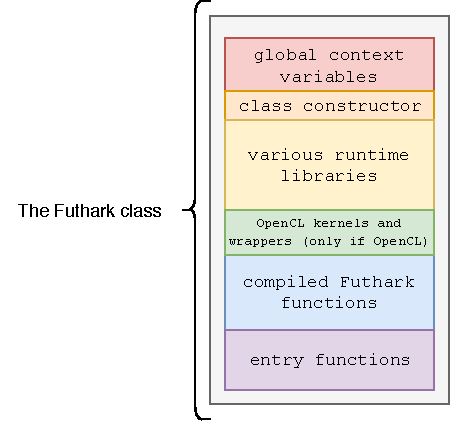
\includegraphics{chapters/figs/csharp/futhark_class.pdf}
  \caption{An overview of the Futhark class}
  \label{fig:futharkclass}
\end{figure}


\subsubsection{Global context variables}
\label{globalcontextvariables}
Compiled Futhark programs need to keep track of several variables.
Both normal and OpenCL-enabled Futhark \csharp{} programs can take several
options when they're launched from the command line. For example,
\texttt{num\_runs} tells the Futhark runtime how many times the chosen entry
function should be executed, and the variable \texttt{runtime\_file} tells the
Futhark runtime where it should write timing information to, for example for
benchmarking purposes.

Instead of passing an argument array along throughout all the functions in the
Futhark class, like we usually would do if we were writing purely functional
programs, we instead represent these arguments as class variables, which 
are set when the class is instantiated. 
This allows to refer to them from wherever in the rest of the class
(without passing them explicitly as arguments).

For non-OpenCL programs, these variables are exclusively used for benchmarking and
debugging purposes. For OpenCL programs however, the global variables are vital
for the program's execution.
In an OpenCL program, the Futhark class must keep track of two extra
variables.

The first variable is \texttt{struct futhark\_context ctx} and contains 
the global state of the current program's execution. The global state consists of 
\begin{itemize}
    \item[(1)] the current list of unused but allocated OpenCL buffers on the device, 
    \item[(2)] kernel handles for all the OpenCL kernels used in the Futhark program,
    \item[(3)] a counter for the total running time of the program.
    \item[(4)] the  \texttt{opencl\_context}, which holds the metadata necessary for
                OpenCL execution, for example the current state of the device, 
                the queue of in-execution OpenCL actions, and so forth.
\end{itemize}

The second variable is \texttt{struct futhark\_context\_config cfg} and records
configuration information necessary for constructing the actual 
\texttt{futhark\_context}.

\subsubsection{The class constructor}
The class constructor is necessary to setup the global variables needed
throughout the Futhark class. When the Futhark program is compiled as an
executable, the command line arguments are passed to the class constructor by
the \texttt{Program} class. If the Futhark program is compiled as a library, the
programmer can pass a string array of arguments to this constructor manually.

Besides setting class variables, OpenCL-enabled versions will initialize (and
set) first the \texttt{futhark\_context\_config cfg} variable, and afterwards
the \texttt{futhark\_context} itself.

\subsubsection{The various runtime libraries}
\label{subsec:runtimelibs}

The runtime libraries are a set of seperate \csharp{} files that are written and
distributed through the Futhark compiler. When a Futhark program is compiled,
these library files are concatenated and embedded directly into the rest of the
generated code. They contain functionality which the generated Futhark programs
depend on.
The runtime libraries are the following:
\begin{description}
\item[\texttt{memory.cs}] \hfill\\
  Futhark's imperative IR ({\tt ImpCode}) represents all arrays---no matter of 
    their dimensionality and primitive-element type---as a flat one-dimensional 
    array of bytes, which are accompanied by an array of 64-bits integers 
    recording the dimensions of the flat array.  As such it was necessary to 
    define a set of functions that are able to interact with these byte arrays,
    e.g., if the original array was holding {\tt float}s, than we need to be
    able to read/write a float value from/into the byte array. 
  For example, \texttt{memory.cs} contains the \texttt{writeScalarArray} functions,
  which writes a scalar value to a certain location into the byte array. The 
    function is overloaded so it works with scalars of any integer or floating 
    point primitive types. Figure~\ref{fig:writeScalarArray} shows the instance
    of {\tt writeScalarArray} that writes a value of type {\tt double} into the
    byte array.
\begin{figure}[h]
\centering
\begin{minted}[fontsize=\small]{csharp}
void writeScalarArray(byte[] dest, int offset, double value)
{
    unsafe
    {
        fixed (byte* dest_ptr = &dest[offset])
        {
            *(double*) dest_ptr = value;
        }
    }
}
\end{minted}
\caption{\texttt{writeScalarArray} writes a value at the specified offset in
some byte array.}
\label{fig:writeScalarArray}
\end{figure}

\item[\texttt{scalar.cs}] \hfill\\
  This library contains all the scalar functions necessary for Futhark \csharp{}
  programs.
  In Futhark, arithmetic operators are defined for integers and floats of all
  sizes, and bitwise operators are defined for all integers.
  However, this is not the case in \csharp{}, where many arithmetic operators
  are only defined for 32- and 64 bit integers.
  
  If these operators are used with 8- or 16 bit operands, the operands are
  implicitly casted to 32 bit integers at compile time, which also means that
  the final result of the operation is a 32 bit integer, which doesn't has the
  right type.

  Therefore, wrapper functions must be defined for even the simplest arithmetic
  functions. For example, integer addition in \csharp{} Futhark is actually
    implemented by four different functions:
\begin{minted}[fontsize=\small]{csharp}
static sbyte add8(sbyte x, sbyte y){ return Convert.ToSByte(x + y); }
static short add16(short x, short y){ return Convert.ToInt16(x + y); }
static int add32(int x, int y){ return x + y; }
static long add64(long x, long y){ return x + y; }
\end{minted}

  Besides, \texttt{scalar.cs} also contains the \csharp{} definitions for the various
  mathematical functions from Futhark's \texttt{math.fut}library, such as \texttt{exp},
  \texttt{sin} and \texttt{cos}.


\item[\texttt{reader.cs}] \hfill\\
  The reader contains the entire functionality for recieving function parameters
  through \texttt{stdin}, as shown in the example in subsec
  \ref{subsec:futharkcsexe}.
  The reader reads scalars of any of the Futhark-supported primitives, and also arrays and multidimensional arrays of scalars.

  The reader also supports reading streams of binary data. This enables Futhark
  to parse datasets that are stored as pure byte representation, instead of
  string representations.
  It is only necessary for Futhark executables.
  

\item[\texttt{opencl.cs}] \hfill\\
  \texttt{opencl.cs} contains wrapper functions for \texttt{OpenCL}'s memory
  related functions. For example, instead of calling \texttt{clCreateBuffer} directly for
  allocating an \texttt{OpenCL} buffer, we call \texttt{OpenCLAlloc} from
  \texttt{opencl.cs}. By using a wrapper function instead of calling
  \texttt{clCreateBuffer}, we encapsulate functionality and employ better error
  handling.
  The wrapper functions in \texttt{opencl.cs} also employs a \texttt{free list} for \texttt{OpenCL}
  memory allocations. This list is stored in the \texttt{futhark\_context}, and
  has the following functionality:
  \\
  1) When the Futhark program frees an \texttt{OpenCL} buffer, it is not
  actually freed, but is instead added to the \texttt{free list}.\\
  2) When the Futhark program later allocates an \texttt{OpenCL} buffer, it
  first goes through the \texttt{free list} to see, whether it can use one of the already
  existing allocations instead.
\end{description}

\subsubsection{The compiled Futhark functions}
  The compiled Futhark functions are the Futhark functions as written in
  \texttt{ImpCode}\footnote{See figure \ref{fig:impcode}}, expressed in the
  target language, in this case \csharp{}.

  The compiled Futhark functions corresponds to the entry functions found
  in the entry functions-section of the Futhark class.
  Only the Futhark \texttt{entry} functions are compiled to individual functions, and
  remaining helper functions are inlined here.

  In OpenCL programs, all array functions and SOAC calls are compiled as
  individual (or fused) OpenCL kernels. Therefore, the compiled Futhark
  functions in these programs consists of mainly some scalar operations and
  memory allocations, and calls to Futhark-generated kernel wrapper functions.
  There are also mixes, for example \texttt{for-}loops that call OpenCL kernels.
  
  In non-OpenCL programs, the array functions and SOAC calls are not stored in
  seperate wrapper functions, but inlined in the Futhark functions.

\subsubsection{OpenCL kernels and wrappers}
  If the Futhark program is compiled for OpenCL, all array handling function- and
  SOAC calls are compiled as OpenCL kernels. This part of the Futhark class
  has two parts:
  \begin{enumerate}
  \item The string (actually a single string in an array) \texttt{opencl\_prog}, which contains the entire
  Futhark-generated OpenCL source code for the Futhark program in question.
  This source code contains all the OpenCL kernels for the program, and is
  passed to the OpenCL device, compiled and loaded, when the Futhark class is
  initialized. Handles to the individual kernels are then stored in the \texttt{futhark\_context}.

  \item For each kernel in the \texttt{opencl\_prog}, the Futhark compiler
    generates a kernel wrapper function. These wrapper functions takes the
    kernel arguments (such as scalar values, array values and indexes) as input,
    and performs all the OpenCL specific work necessary for the actual kernel
    launch; for example setting the kernel arguments on the device, and copying
    data back and forth between host and device buffers.
  \end{enumerate}

\subsection{Entry functions}
\label{csharpentries}
Futhark's internal representation of array values are one dimensional byte
arrays (which can represent arrays of any type and dimensionality), and an
accompanying list of integers denoting the lengths of the array's dimensions.
However, Futhark does not expect it's users to pass this form of arrays as
function arguments, which is why each Futhark \texttt{entry} function has a
corresponding entry function in the final compiled code.
\\\\
To discern between Futhark functions and entry functions, the Futhark function's
name is prefixed with ``\texttt{futhark\_}'', as in for example
``\texttt{futhark\_foo}''.
Depending on whether the Futhark program is compiled as an executable or a
library, the entry function itself is then named ``\texttt{entry\_foo}'' or
just ``\texttt{foo}''.

For executables, ``\texttt{entry\_foo}'' is a function that doesn't take any
arguments. Instead, it uses the reader functions from \texttt{reader.cs} to parse the
arguments for ``\texttt{foo}'' from \texttt{stdin}, and passes them to the
Futhark function. For all array values in the arguments, the array values are
converted into Futhark representations of them.
When the Futhark function returns the result, the result is then printed to \texttt{stdout}.

\subsection{Entry functions in executables}
\label{entryfunctionsinexecutables}
Consider again our small Futhark program mapPlus2 (figure \ref{fig:mapplus20}).
\begin{figure}[H]
  \centering
  \begin{lstlisting}[language=Futhark]
entry main (xs : []i32) : []i32 =
  map (+2) xs
  \end{lstlisting}
  \caption{A short Futhark program called mapPlus2.fut}
  \label{fig:mapplus20}
\end{figure}

If we compile this program as an executable, we get Futhark/entry function pair
shown in figure \ref{fig:futharkentrypairexe}. The example is very simplified
but does resembles the actual implementation in functionality.

By calling \texttt{entry\_main()}, we first call \texttt{ReadStrArray<int>} to parse an integers
array from stdin. We then read the number of elements in the array into a
variable, and then convert the integer array to a byte array, as Futhark
functions use byte arrays for internal value array representation.

We then call the internal Futhark function, which returns a byte array, the
length of the byte array and the number of elements that the byte array
represents.
We reform the byte array into an integer array, and print the result to \texttt{stdout}.

\begin{figure}[H]
  \centering
\begin{minted}[linenos, breaklines]{csharp}
(int, byte[], int) futhark_main(int byte_array_length, byte[] byte_array, int byte_array_elms)
{

    // ...
    // futhark stuff happens
    // ...

    return (out_array_length, out_array, out_array_elms);
}

void entry_main()
{
    var (int_array, lengths) = ReadStrArray<int>(1, "i32");
    var int_array_elms = lengths[0];
    var byte_array = convertToByteArray<int>(int_array);
    var byte_array_length = byte_array.Length;

    var (res_array_memsize, res_array, res_array_elms) =
        futhark_entry(byte_array_length, byte_array, int_array_elms);

    var res_array_as_ints = reform_array<int>(res_array, res_array_elms);
    printArray(res_array_as_ints);
    exit(0);
\end{minted}
  \caption{A simplified Futhark/entry function pair from the mapPlus2 executable}
  \label{fig:futharkentrypairexe}
\end{figure}

\subsection{Entry functions in libraries}
If we compile the program in fig \ref{fig:mapplus20} program as a library, we get Futhark/entry function pair
shown in figure \ref{fig:futharkentrypairlib}. The example is very simplified
but does resembles the actual implementation in functionality.

The difference between this example and the example in 
section~\ref{entryfunctionsinexecutables} is that the arguments of the Futhark export
are passed directly to the wrapper (e.g., {\tt entry\_main}) instead of being parsed
from {\tt stdin}. Similarly, the result of the wrapper is the type-casted result of
the Futhark export as opposed to the result being written to \texttt{stdout}.
\begin{figure}[H]
  \centering
\begin{minted}[linenos, breaklines]{csharp}
    (int, byte[], int) futhark_main(int byte_array_length, byte[] byte_array, int byte_array_elms)
    {

        // ...
        // futhark stuff happens
        // ...

        return (out_array_length, out_array, out_array_elms);
    }

    (int[], int[]) entry_main(int[] int_array, int[] int_array_lengths)
    {
        var int_array_elms = int_array_lengths[0];
        var byte_array = convertToByteArray<int>(int_array);
        var byte_array_length = byte_array.Length;

        var (res_array_memsize, res_array, res_array_elms) =
            futhark_entry(byte_array_length, byte_array, int_array_elms);

        var res_array_as_ints = reform_array<int>(res_array, res_array_elms);
        var res_lengths = new int[] { res_array_as_ints.Length };
        return (res_array_as_ints, res_lengths);
\end{minted}
  \caption{A simplified Futhark/entry function pair from the mapPlus2 library}
  \label{fig:futharkentrypairlib}
\end{figure}

\subsection{On calling Futhark entry functions that takes arrays as arguments}
\label{subsec:flatarraysinentryfuncs}
Currently, library functions aren't callable with jagged arrays (arrays of 
pointers to arrays), but must instead be called with a flat element array,
which is paired up with an array of lengths denoting the dimensionality of 
the flat element array. This is explained in sec \ref{sec:convertingarrays}.

The \fshark{} implementation offers helper functions that can flatten jagged
arrays into flat arrays/dimension array pairs, and back again.
In the future, this might be added to the Futhark \csharp{} backend for
usability purposes.

\subsection{The Program class design}
\label{subsec:programclass}
As shown in figure \ref{fig:futharkcsclasses}, we only add the Program class to
the Futhark program so we have an entrypoint for the executable.

The Program class is a \csharp{} necessity for compiling executable \csharp{}
programs, as the \csharp{} standard demands that executable programs must have a
\texttt{Program} class with a public \texttt{Main} method, that it can use as an
entrypoint.
In Futhark's case, the Main method initializes the internal Futhark class and
calls the entry function in the class. The class is shown in the figure
below:

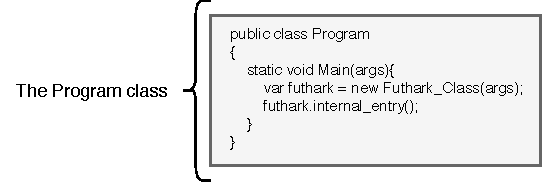
\includegraphics{chapters/figs/csharp/program_class.pdf}

%%% \section*{The \csharp{} backend, compared to the C- and Python counterparts}
%%% 
%%% %% DESCRIBE THE DIFFERENCES BETWEEN C# AND THE REST
%%% THE PYTHON BACKEND HAS MUCH FUNCTIONALITY ENCAPSULATED IN PYOPENCL, AND DOESN'T
%%% NEED TO DECLARE VARIABLES BEFORE SETTING THEM
%%% LESS COMPLEX GENERATOR NEEDED AS VARIOUS OPENCL STATEMENTS ARE HANDLED
%%% AUTOMATICALLY BY LIBRARY
%%% 
%%% C BACKEND MUST BE AWARE OF ALL SIZES AND EVERYTHING AT COMPILE TIME, WHICH MEANS
%%% STATES MUST BE ALLOCATED THROUGH COMPLEX STRUCTS AT COMPILE TIME, AND STRUCTS
%%% MUST BE DEFINED AT COMPILE TIME AS WELL
%%% 
%%% C ALLOWS NULL POINTERS, CS DOES NOT WHICH MEANS WE NEED PLACEHOLDER VARIABLES
%%% 
%%% CSHARP GENERATOR IS SOMEWHERE INBETWEEN AS IT IS CAN HANDLE OBJECTS WHICH CAN
%%% CARRY STATE, FURTHERMORE DYNAMIC MEMORY ALLOCATION
%%% 
% THE DIFFERENCES BETWEEN MEMORY HANDLING IN CS AND CSOPENCL
\section{Memory management in Futhark \csharp{}}
As Futhark stores array values in byte arrays, it is relevant to compare
the difference between how the array handling differs between Futhark's C
backend, and this \csharp{} backend.
For OpenCL programs, the memory management of \csharp{} and C is largely the
same, as the OpenCL side of these programs are the same. \csharp{} does after
all just use C bindings for it's OpenCL interactions.

However, for non-OpenCL \csharp{} programs, we have to take \csharp{}'s memory
model into consideration.

C implicitly allows unsafe programming. In this case, it means interacting with system
memory by reading and writing arbitrary values from/to arbitrary locations,
designating the values and destinations as whatever type we want.
In figure \ref{fig:futharkcscene}, we see a \texttt{for}-loop that
performs a prefix-sum operation on an array of integers.
On line 6, reading from right to left, we are first creating a reference to
a location in the byte array \texttt{xs\_mem\_4223}. However, as the reference
is a pointer to a byte in the array, we must recast it as an \texttt{int32\_t} pointer.
After we do this, we can finally dereference the pointer to retrieve a four byte
integer from the byte array.

We add the retrieved integer to our accumulating variable
\texttt{scanacc\_4187}, before we cast a reference in our destination byte array
as an integer pointer, and store the result there.

\begin{figure}
\centering
\begin{minted}[linenos, fontsize=\small]{c}
memblock mem_4226;
memblock_alloc(&mem_4226, bytes_4224);
int32_t scanacc_4187 = 0;

for (int32_t i_4189 = 0; i_4189 < sizze_4135; i_4189++) {
    int32_t x_4147 = *(int32_t *) &xs_mem_4223[i_4189 * 4];
    
    scanacc_4187 += x_4147;

    *(int32_t *) &mem_4226[i_4189 * 4] = scanacc_4187;
}
\end{minted}
\caption{A short snippet from a Futhark C program}
\label{fig:futharkcscene}
\end{figure} 

In \csharp{}, arrays and lists are accessed by indexing, for example \texttt{var
  x = myArray[10];}.
These arrays are managed by .NET's CLR\footnote{Common Language Runtime}, and
access violations, such as indexing out of bounds, makes the CLR raise a suitable
exception, which can be handled in the \csharp{} program by catching it
accordingly.

However, for performance reasons\ref{marshalunsafeperformance}, we are 
interested in writing to our \csharp{} arrays directly.
To do this, we must use both \texttt{unsafe} blocks and \texttt{fixed} blocks.
Note that this does not necessarily result in unsafe code, because the Futhark
generated code is performing the safety checks already.

\subsubsection{The \texttt{unsafe} block}
In \csharp{}, we cannot just write arbitrary values to arbitrary locations, as this
opens the program for memory access violations by trying to access memory
outside of \csharp{}s memory space. Such violations triggers segmentation faults
which halts the entire program, instead of throwing an exception.

Therefore we encapsulate our unsafe pointer-using code in an \texttt{unsafe}
block.

\subsubsection{The \texttt{fixed} block}
\csharp{}s CLR manages memory locations for allocated buffers, which means that
it also moves these memory allocations around in memory during program execution
when necessary.
To be able to read and write to buffers referenced by pointers, we must
therefore fix these buffers in memory, before we are able to use them directly.

An example of using the unsafe- and the fixed block is shown in figure
\ref{fig:writeScalarArray'}. We start the function by starting an
\texttt{unsafe} block. After we have started the \texttt{unsafe} block, we fix
the destination buffer in memory and get a pointer to the exact location that we
are interested in. Finally, we use a cast to treat the destination pointer as a
\texttt{double} pointer so we can store a \texttt{double} at that location.
\begin{figure}[h]
\centering
\begin{minted}[fontsize=\small]{csharp}
void writeScalarArray(byte[] dest, int offset, double value)
{
    unsafe
    {
        fixed (byte* dest_ptr = &dest[offset])
        {
            *(double*) dest_ptr = value;
        }
    }
}
\end{minted}
\caption{\texttt{writeScalarArray} writes a value at the specified offset in
some byte array.}
\label{fig:writeScalarArray'}
\end{figure}

\subsection{Performance}
\label{marshalunsafeperformance}
Although \csharp{} does offer safe methods to store values directly in byte
arrays, we have chosen to avoid these functions as their implementations carry
huge overhead compared to doing things the unsafe way.
For this benchmark, we are writing N integers to a byte array, using the three
methods shown in figure \ref{fig:threemethods}.
\begin{figure}
  \centering
  \begin{minted}{csharp}
static void UsingBuffer()
{
    byte[] target = new byte[TEST_SIZE*sizeof(int)];
    for (int i = 0; i < TEST_SIZE; i++)
    {
        var intAsBytes = BitConverter.GetBytes(i);
        Buffer.BlockCopy(intAsBytes, 0, target, i * sizeof(int), sizeof(int)); 
    }
}

static void UsingUnsafe1()
{
    byte[] target = new byte[TEST_SIZE*sizeof(int)];
    for (int i = 0; i < TEST_SIZE; i++)
    {
        unsafe
        {
            fixed (byte* ptr = &target[i * sizeof(int)])
            {
                *(int*) ptr = i;
            }
        }
    }
}

static void UsingUnsafe2()
{
    byte[] target = new byte[TEST_SIZE*sizeof(int)];
    unsafe
    {
        fixed (byte* ptr = &target[0])
        {
            for (int i = 0; i < TEST_SIZE; i++)
            {
                *(int*) (ptr+i*sizeof(int)) = i;
            }
        }
    }
}

\end{minted}
  \caption{Three methods of writing integers to an array.}
  \label{fig:threemethods}
\end{figure}


The full program is available in listing \ref{fig:memoryperformancebenchmark} in the
appendix, to compare safe and unsafe methods of writing values to byte arrays, and the
results (as shown in fig \ref{fig:shortperformancegraph}) tells us that there
are definite performance gains to retreive by going \texttt{unsafe}.

The obvious reason for the performance difference is, that for the safe
method, in each of the N iterations, the BitConverter allocates a small 
array of bytes, where the value of integer-scalar {\tt i} is recorded,
and then it copies this small array into the target byte array. 
The unsafe methods do not exhibit this overhead, since they update directly
the target byte array. 
The performance difference between the second and third method corresponds to
the small overhead that comes from fixing the target buffer in memory.

\begin{figure}
    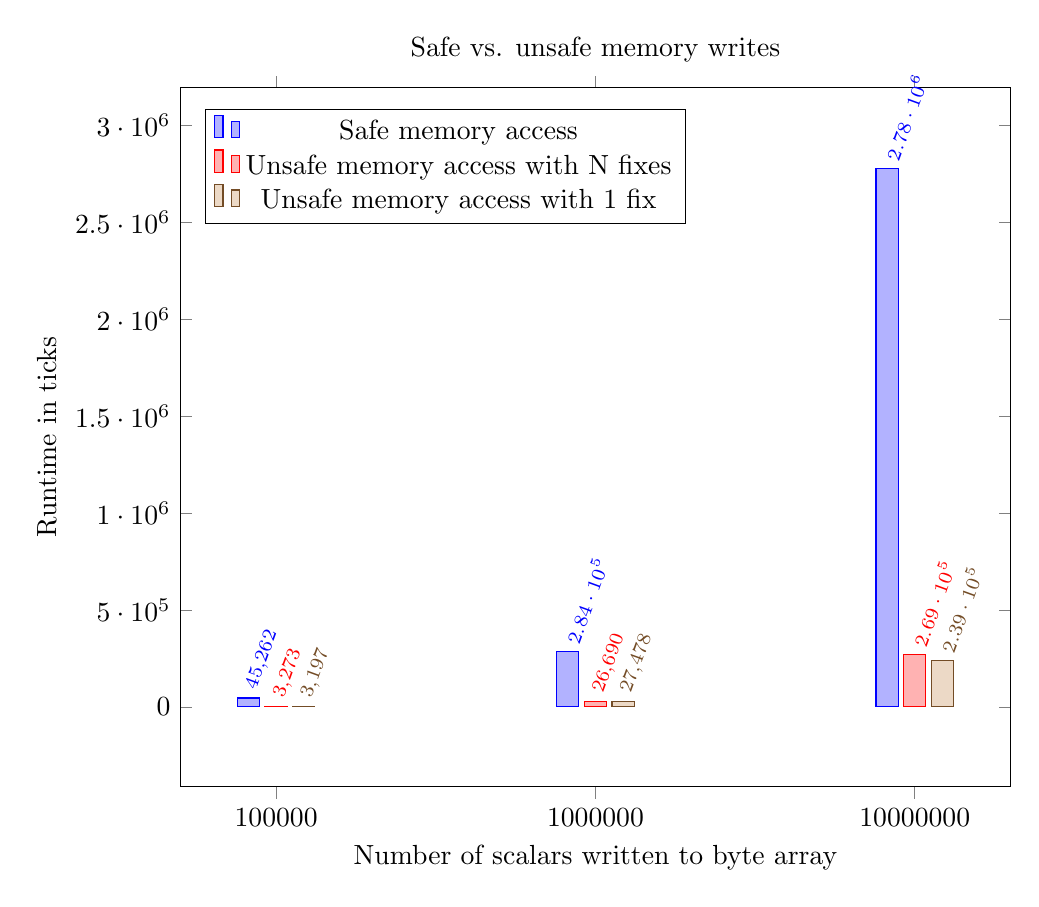
\begin{tikzpicture}
      \begin{axis}[
        title={Safe vs. unsafe memory writes},
        xlabel={Number of scalars written to byte array},
        ylabel={Runtime in ticks},
        width=1\textwidth,
        %height=0.5,
        scaled y ticks=false,
        symbolic x coords={100000, 1000000, 10000000},
        xtick=data,
        enlargelimits=0.15,
        ybar=2pt,% configures ‘bar shift’
        bar width=8pt,
        nodes near coords,
        every node near coord/.append style={rotate=70, anchor=west,font=\scriptsize},
        legend style={legend pos=north west}
      ]
      \addplot plot coordinates {(100000, 45262 ) (1000000, 284379) (10000000, 2778424)};
      \addplot plot coordinates {(100000, 3273 ) (1000000, 26690) (10000000, 268978)};
      \addplot plot coordinates {(100000, 3197 ) (1000000, 27478) (10000000, 238691)};
      \legend{Safe memory access, Unsafe memory access with N fixes, Unsafe memory access with 1 fix}
      \end{axis}
    \end{tikzpicture}
    \caption{Comparison between safe and unsafe methods for writing scalars in a byte array.}
    \label{fig:shortperformancegraph}
\end{figure}

\section{Selecting an OpenCL interface for \csharp{}}
OpenCL interaction is not a part of the .NET standard library, but several
libraries do exist for .NET/OpenCL interactions. For this thesis, I researched a
selection of these libraries, to determine which one that would fit the best for
my purposes.
As Futhark depends on being able to interface with the OpenCL platform directly,
it was necessary to find an OpenCL library for .NET which had direct bindings to
the OpenCL developer library.

The .NET libraries I took into consideration was \texttt{NOpenCL}, \texttt{OpenCL.NET} and \texttt{Cloo}.
All three libraries have been designed to aide OpenCL usage in \csharp{}
programs, by simplifying OpenCL calls behind abstractions, for example by
wrapping pointer operations in private methods.
\\
\\

\begin{description}
\item[\texttt{NOpenCL}]\hfill\\
\texttt{NOpenCL} was the first candidate for the \csharp{} backend, and had
several advantages to the other two: As per February 2018, it had been updated
within the last year, and was therefore the least deprecated library. Second,
the \texttt{NOpenCL} repository on Github contains both unit tests and
example programs.

However, \texttt{NOpenCL} is also tailored for Windows use, and therefore not a
good fit for Futhark, as Futhark is available on both Windows, Linux and Mac OS.
Furthermore, the library is not available through the NuGet
package manager, and the OpenCL API calls are needlessly complex to work with
through the library.

\item[\texttt{OpenCL.NET}]\hfill\\
\texttt{OpenCL.NET} also has a test suite, is available through NuGet, and is
used as the backend for other libraries, such as the \fsharp{} GPU library
\texttt{Brahma.FSharp}.

However, this library hardcoded to work on a in a Windows context, and has not been
updated for more than five years.

\item[\texttt{Cloo}]\hfill\\
\texttt{Cloo} is usable on all three
platforms, and it is available on NuGet. Furthermore, as opposed to the other two libraries, the
Cloo library contains a class with static functions that does nothing but
passing arguments on to the OpenCL library, using \csharp{}s \texttt{DllImport}
attribute. It is immediately possible to skip most of \texttt{Cloo}s features,
and just use the library for it's OpenCL bindings.

Furthermore, the \texttt{Cloo} project is still alive, and the \texttt{Cloo}
\texttt{develop} branch on Github is actively being updated as per July 2018\footnote{\url{https://github.com/clSharp/Cloo/commits/develop/Cloo/Source}}.
\\
\\
\end{description}
Given these three candidates, I chose to work with \texttt{Cloo}: It was the
only one that had the necessary OpenCL bindings readily available, and the only
one that was platform agnostic.
%%% Local Variables:
%%% mode: latex
%%% TeX-master: "../thesis"
%%% End:

\chapter{Benchmarks and evaluation}
SPECS HERE

%%% Local Variables:
%%% mode: latex
%%% TeX-master: "../thesis"
%%% End:
\chapter{Current limitations}
In the chapter, we describe the current known limitations of both our code
generator, the \fshark{} language design and of the \fshark{} compiler. The
limitations are divided into two categories; those caused by our design choices,
and those caused by a lacking implementation.

\section{The \csharp{} code generator}
Both of the code generator limitations listed below are caused by lack of
implementation.

\subsection{Cumbersome array entry functions in Futhark libraries}
\label{cumbersomearrays}
As described in sec. \ref{subsec:flatarraysinentryfuncs}, we currently have to
flatten our jagged arrays before we can pass them to our Futhark library
functions. Likewise, we have to unflatten the results if we want to use them as
jagged arrays again afterwards.

In sec. \ref{sec:convertingarrays}, we presented a solution for both flattening
and unflattening such arrays, and thus solving this limitation is merely a
question of porting and implementing these algorithms in the Futhark generated
\csharp{} libraries.

\subsection{Unnecessary memory allocations in chained Futhark function calls}
The current implementation of the code generator causes significant overhead
when chaining together GPU function calls, as discussed in sec.
\ref{invocationoverhead}.
Whilst not being a functional limitation, implementing an
opaque return type for Futhark GPU calls would increase runtime
performance in any programs that chain together such calls.

The Python code generator for Futhark already has such an opaque data type
implemented, and one could look to this implementation for inspiration on how to
design a similar data type for Futhark \csharp{}.

\section{The \fshark{} language}


\section{The \fshark{} compiler}

\subsection{Disallowing certain types of \fshark{} entry functions}
As the \fshark{} wrapper relies on the flattening algorithms shown in sec.
\ref{sec:convertingarrays} to make \fsharp{}s jagged arrays compatible with
Futhark's flat arrays (sec. \ref{subsec:flatarraysinentryfuncs}), we currently
prohibit \fshark{} entry functions have return types that are either
\texttt{('a[] * int64[])} tuples, or tuples or arrays that contains such
tuples. This is described in detail in subsec. \ref{subsec:hinderedtupletype}.

This could be solved by moving the array flattening into the generated Futhark
\csharp{} libraries as described in subsec. \ref{cumbersomearrays}, solving two
limitations at the same time.


%%% Local Variables:
%%% mode: latex
%%% TeX-master: "../thesis"
%%% End:

\chapter{Method}

%%% Local Variables:
%%% mode: latex
%%% TeX-master: "../thesis"
%%% End:

\chapter{Related work}

%%% Local Variables:
%%% mode: latex
%%% TeX-master: "../thesis"
%%% End:

\chapter{Conclusion and future work}

%%% Local Variables:
%%% mode: latex
%%% TeX-master: "../thesis"
%%% End:
\include{chapters/a_appendices}
\chapter{Array handling in FShark}
% introduction
\fsharp{} is a functional programming language on top of the .NET framework, which
means that it's primitive types like \texttt{int, float} and \texttt{list} all
correspond to already existing classes in the .NET framework. For example,
\fsharp{}'s \texttt{int} is an alias for .NET's \texttt{System.Int32} and
\texttt{float} is an alias for \texttt{System.Double}.

Therefore, we also find corresponding .NET classes for both \fsharp{}
\texttt{list}s and \texttt{array}s. \texttt{list}s are
\texttt{FSharp.Collections.FSharpList}s, and \texttt{array}s are
\texttt{System.Array}. (Note that \texttt{FSharpList}s is available from any
.NET framework language, as long as the corresponding assembly is referenced).

Although it is common to use lists in functional programs, the \fsharp{} subset
covered by FShark does not include lists -- In Futhark, and therefore also
FShark, our main goal is not handling list elements one after another, but
rather parallelizing computations across entire arrays of data simultaneously.

The \texttt{FSharp.Collections.FSharpList} is implemented as a singly-linked
list. SOACs called on singly-linked lists are inherently unparallelizable, as
the SOACs must traverse the list sequentially.
For example, calling $\texttt{map} f$ on a singly linked list \texttt{(x::xs)}
means computing $f \texttt{x}$ and inserting the result into $\texttt{map} f
\texttt{xs}$ recursively. We can do some parallel computations for these kinds
of SOACs, i.e. by making the main thread traverse the list and spawn
a thread for each element computation. However we will still have suboptimal
memory access performance, as the elements in the singly linked list doesn't
have any guarantees regarding their location in RAM, which means we are going to
perform many more memory loads compared to if we were performing calculations on
elements in a sequentially stored array elements in RAM.


% a basic description of lists in F# and arrays in F#

% short description of multidims in F#
% description of jagged arrays in F#
% description of array handling in Futhark 

% a description of SOACs in FSharkPrelude, analysis of various time complexities
% for FSharkPrelude SOACs

%% handling irregular arrays at runtime when using FSharkPrelude.

% Wrapping and unwrapping when invoking functions:
%% Why do we need to completely flatten arrays before passing into Futhark
%% module?
%%% Array flattening algorithm in pseudocode
%%% Cost of algorithm


% Reshaping flat array into jagged array
%% Description of algorithm
%% Cost of algorithm

% performance??

% alternative solutions: FSharkArrays

%%% Local Variables:
%%% mode: latex
%%% TeX-master: "../thesis"
%%% End:
\chapter{\fshark{}s interoperability between \fsharp and Futhark (\csharp{})}
FShark stands on three legs: The FShark compiler, the Futhark C\# code generator, and
the FSharkWrapper.
The compiler is responsible for compiling FShark source code into Futhark
source code, and the C\# code generator takes the result Futhark source code,
and compiles OpenCL powered C\# libraries, which can be imported directly back
into F\#.

It is of course possible to use the compiler and the code generator as
individual modules, but for this project, the FSharkWrapper has been designed to
let users use FShark without having to understand any of the underlying
pipeline.

To illustrate this; take a look at figure \ref{fig:fsharkusingwrapper}. In the
first line, the user initializes the FSharkWrapper with the arguments necessary
to use the wrapper itself. In the second line, the user adds a source file to
the wrapper by it's path.
In the third line, the user tells the wrapper to run the compilation pipeline.
Assuming that the compilation goes well, the user can then invoke some function
from the FShark program in line four.

Here, calling the \texttt{CompileAndLoad()} function triggers the entire \fshark{}
pipeline as described in \ref{pipeline}, and does then have a function available
for the user to call afterwards.

However, as this is the default way of using \fshark{}, we are currently calling
\texttt{CompileAndLoad()} every time we use the \fshark{} program.
This is happening even though we only need the final compiled C\# assembly to
load back into \fsharp{} at runtime. 

Everytime we run the FShark compiler pipeline, we are therefore also
\begin{enumerate}
\item parsing, typechecking and generating a TAST from the \fshark{} code,
  using FSharp's compiler.
\item generating Futhark source code from the FSharp TAST
\item Writing the Futhark source code to disk
\item running the Futhark compiler and C\# code generator on the Futhark source
  code
\item running the mono C\# compiler on the resulting C\# source code
\end{enumerate}

For two selected benchmarks we have the following times
% Numbers for nbody.fut:
%  FShark parsing took 1850345 ms
%  FSharpDecls to FSharkIL took 76660 ms
%  FSharkIL to Futhark source code took 43471 ms
%  Compiling the Futhark module into .cs source code took 1555105 ms
%  Compiling .cs module took 999251 ms
%  Loading compiled .cs assembly using reflection took 101601 ms
%  The entire FShark compilation pipeline took 4634460 ms
%  Average invokation time was 104227 ms
%  Invoking main took 107597 ms

% LocVolCalib.fut small
%FShark parsing took 217984 ms
%FSharpDecls to FSharkIL took 19129 ms
%FSharkIL to Futhark source code took 98949 ms
%Compiling the Futhark module into .cs source code took 8037165 ms
%Compiling .cs module took 1422527 ms
%Loading compiled .cs assembly using reflection took 81370 ms
%The entire FShark compilation pipeline took 9877907 ms
%Average invokation time was 219150 ms
%
% locvolcalib medium
% FShark parsing took 221395 ms
% FSharpDecls to FSharkIL took 21487 ms
% FSharkIL to Futhark source code took 107558 ms
% Compiling the Futhark module into .cs source code took 7739211 ms
% Compiling .cs module took 1467667 ms
% Loading compiled .cs assembly using reflection took 77850 ms
% The entire FShark compilation pipeline took 9635733 ms
% Average invokation time was 333960 ms
% 
% locvolcalib large
% FShark parsing took 229771 ms
% FSharpDecls to FSharkIL took 20973 ms
% FSharkIL to Futhark source code took 111219 ms
% Compiling the Futhark module into .cs source code took 7452111 ms
% Compiling .cs module took 1422789 ms
% Loading compiled .cs assembly using reflection took 79751 ms
% The entire FShark compilation pipeline took 9317354 ms
% Average invokation time was 5863264 ms

% nbody from assembly:
% Opening class from assembly took 61841 ms
% Running nbody from assembly took 117373 ms

% locvolcalib
% small
% Opening class from assembly took 147341 ms
% Running locvol small from assembly took 210698 ms
% medium
% Opening class from assembly took 61771 ms
% Running locvol medium from assembly took 314444 ms
% large
% Opening class from assembly took 71198 ms




% make a chart that shows the time consumption of a regular FShark execution
% (for LocVolCalib and nbody) from start to finish, and what the time is spent
% on 

% make the same chart but where the assembly is referenced at compile time,
% which means that the FShark program is just used as a compiler.

% for both tests, we use ArrayToFlatArray, as we have still settled on normal
% arrays as the array.

\subsection{Pros and cons of the current design}
As there are demonstratively great performance gains to be won by only using the
compiler part of the FShark pipeline, it is worth discussing whether the
rest of the FShark pipeline should remain.

Besides eliminating the entire compilation operation at every \fshark{}
execution, a compiler-only approach to the \fshark{} compiler would give us the
following advantages:
\begin{itemize}
\item \textbf{Standalone-modules first:} As the compiler is now only
  used once, the resulting Futhark assembly is readily importable in any .NET
  project, as long as the required Mono libraries are also available.
  This goes not only for the user who just compiled the assembly, but also for
  any other user who has acquired the necessary Mono libraries. This means that
  the \fshark{} developer can use and share the \fshark{} assemblies with
  colleagues and coworkers like any other sharable .NET library,
  as this is indeed what a compiled Futhark
  \csharp{} library amounts to.

  Corollarily; this \fshark{} design would make \fshark{} is useful for generating
  high-performing .NET libraries. (Although one could write such libraries in
  Futhark instead of \fshark{}.)

\item \textbf{Static typing of \fshark{} module:} The current runtime-only
  approach means that the user must rely on reflection to call \fshark{}
  functions.
  In this situation, all modern IDE comforts like autocompletion, and especially
  static type checking and inference falls away.
  For the following example
  %% let foo (x : int) ((y,z) : (int * int)) : (int * int) 
  , the current design demands that we first wrap our arguments in an
  \texttt{obj array}, before invoking the function \texttt{foo}. Furthermore, we
  must also downcast the result using \fsharp{}s downcasting operator \texttt{:?>}.
  Because we are upcasting our arguments to an \texttt{obj array}, we can
  actually pass any (correctly casted) array as an argument to our
  reflection-invoked function, without triggering any type errors at compile
  time.
  The same goes for the downcasted result from the function. We can cast the
  result as whatever type we like, and not run into any trouble until we finally
  run the compiled program.
  % write the example.
  However, if we use \fshark{} to generate assemblies instead, we now have all
  the type information available at compile time. Our compiler will block us
  from compiling the program by giving us useful type errors. Last but not
  least, we can remove all the casting operations that are littering the
  program.
  % other example
  
\item \textbf{Getting rid of, or at least trimming down, the FSharkWrapper:} 
\end{itemize}

However, the current design of \fshark{} also has some advantages that follows
automatically from the design.

\begin{itemize}
\item \textbf{Rapid \fshark{} code development:}
  Currently, it is recommended that any \fshark{} code for a project is also
  built as part of the project.
  By including the \fshark{} file in the original project's source list, we can
  call the \fshark{} module natively, without running the \fshark{} compiler, to
  prototype and debug the \fshark{} code directly in our IDE, before we switch
  to using the compiled version of the \fshark{} code.
  % example of developing
  % 1: picture of placeholder function from Fshark, and fsharp module calling this
  % 2: picture of placeholder function filled out, and fsharp module calling
  % this
  % 3: picture of placeholder function filled out, and fsharp module calling
  % this through fshark

\item \textbf{En mere}
\end{itemize}


% Discuss the pros and cons of the current design:
%% Pros:
%% 1) rapid development. FShark development can take place within the same IDE
%% and project as the FShark-using program.
%% 2) Ease of use: FShark can be used through a few imports and 

%% Cons:
%% 1) Probably the time consumption
%% 2) The need for the FShark wrapper. Because the runtime-only design demands
%% using reflection, the reflection behaviour has been encapsulated in a bulky
%% wrapper object.
\section{The future of \fshark{} interoperability}
With these considerations in mind, my future work on \fshark{}s interoperability
consists of reducing FSharkWrapper in size, so it only takes an \fshark{} source path
  and a .NET assembly outpath as inputs, and does nothing more than
  orchestrating the \fshark{}-, the Futhark- and the \csharp compiler.
  The current design is too complex, largely from supporting too many superflous
  features like concatenating multiple sources, and so on.

I will also be researching the optimal way to keeping the \fshark{} module development as
  close to the rest of the \fshark{}-using project as possible, without %% MERE
  %% HERE
  
The current design enables direct prototyping, which must of course be kept
in later versions of \fshark{}.

%% Another idea: keep annoying wrapper, but let it skip the compiling step.

% \fshark{} as a library generator

%%% Local Variables:
%%% mode: latex
%%% TeX-master: "../thesis"
%%% End:



\end{document}


%%% Local Variables:
%%% coding: utf-8
%%% mode: latex
%%% TeX-command-extra-options: "-shell-escape"
%%% End:
